%-----------------------------------------------------------------------
%
% File Name: thesis.tex
%
% Author: Brown, D. A.
%
% Revision: $Id$
%
%-----------------------------------------------------------------------

% document class and packages
\documentclass[12pt,notitlepage]{report}
\usepackage{bibunits}
%\usepackage{hyperref}
\usepackage{syrthesis}
\usepackage{graphicx}
\usepackage{color}
\usepackage{amsmath}
\usepackage{amssymb}
\usepackage{amsfonts}
\usepackage{rotating}
\usepackage{tensor}

\pdfoutput=1
\DeclareGraphicsExtensions{.pdf,.png}

\hbadness=10000

% new command definitions
\newcommand{\half}{\frac{1}{2}}
\newcommand{\ospsd}{\ensuremath{S_n\left(\left|f_{k}\right|\right)}}

% journal definitions
\newcommand{\apj}{{\it Astrophysical J.}}
\newcommand{\apjl}{{\it Astrophysical J.}}
\newcommand{\aap}{{\it Astron. and Astrophys.}}
\newcommand{\cmp}{{\it Commun. Math. Phys.}}
\newcommand{\grg}{{\it Gen. Rel. Grav.}}
\newcommand{\cqg}{{\it Class. Quant. Grav.}}
\newcommand{\lr}{{\it Living Reviews in Relativity}}
\newcommand{\mnras}{{\it Mon. Not. Roy. Astr. Soc.}}
\newcommand{\pr}{{\it Phys. Rev.}}
\newcommand{\prl}{{\it Phys. Rev. Lett.}}
\newcommand{\prd}{{\it Phys. Rev. D}}
\newcommand{\prsl}{{\it Proc. R. Soc. Lond. A}}
\newcommand{\ptrsl}{{\it Phil. Trans. Roy. Soc. London}}
\newcommand{\rmp}{{\it Rev. Mod. Phys.}}

\begin{document}
\title{% taken from dissertator fellowship application
Topics in Gravitational-Wave Astronomy
}
\author{\bf Prayush Kumar}
\majorprof{Duncan A. Brown}
\submitdate{July 2014}
\degree{Doctor of Philosophy}
\program{Physics}
\copyrightyear{2014}
\majordept{Physics}
\havededicationtrue
\dedication{to\\ the wind and the snow}
\haveminorfalse
\copyrighttrue
\doctoratetrue
\figurespagetrue
\tablespagetrue

\Abstract{% taken from dissertator fellowship application
The Laser Interferometer Gravitational Wave Observatory (LIGO) is one of a new
generation of detectors of gravitational radiation. The existence of
gravitational radiation was first predicted by Einstein in 1916, however
gravitational waves have not yet been directly observed.

One source of gravitation radiation is binary inspiral. Two compact bodies
orbiting each other, such as a pair of black holes, lose energy to
gravitational radiation. As the system loses energy the bodies spiral towards
each other. This causes their orbital speed and the amount of gravitational
radiation to increase, producing a characteristic ``chirp'' waveform in the
LIGO sensitive band.

In this thesis, matched filtering of LIGO science data is used to search for
low mass binary systems in the halo of dark matter surrounding the Milky Way.
Observations of gravitational microlensing events of stars in the Large
Magellanic Cloud suggest that some fraction of the dark matter in the halo may
be in the form of Massive Astrophysical Compact Halo Objects (MACHOs). It has
been proposed that low mass black holes formed in the early universe may be a
component of the MACHO population; some fraction of these black hole MACHOs
will be in binary systems and detectable by LIGO.

The inspiral from a MACHO binary composed of two 0.5 solar mass black holes
enters the LIGO sensitive band around 40 Hz.  The chirp signal increases in
amplitude and frequency, sweeping through the sensitive band to 4400 Hz in 140
seconds. By using evidence from microlensing events and theoretical
predictions of the population an upper limit is placed on the rate of black
hole MACHO inspirals in the galactic halo.
}
\beforepreface
\prefacesection{Preface}
The work presented in this thesis stems from my participation in the LIGO
Scientific Collaboration. 

\vspace*{0.5cm}
\noindent The upper limit on the rate of binary neutron 
star inspirals quoted in chapter \ref{ch:introduction} is based on

\vspace*{0.25cm}

\noindent B.~Abbott~{\it et~al.} (The LIGO Scientific Collaboration),
``Analysis of LIGO data for gravitational waves from binary neutron stars,''
\prd~{\bf 69} (2004) 122001.

\vspace*{0.5cm}

\noindent Chapter \ref{ch:pipeline} is based on material from

\vspace*{0.25cm}

\noindent Duncan A. Brown~{\it et~al.}, ``Searching for Gravitational Waves
from Binary Inspirals with LIGO,'' \cqg~{\bf 21}, S1625 (2004).

\vspace*{0.25cm}

\noindent and

\vspace*{0.25cm}

\noindent B. Abbott~{\it et~al.} (The LIGO Scientific Collaboration), ``Search
for binary neutron star coalescence in the Local Group,'' to be submitted to
\cqg

\vspace*{0.5cm}

\noindent Chapter \ref{ch:hardware} is based on 

\vspace*{0.25cm}

\noindent Duncan A. Brown (for the LIGO Scientific Collaboration), ``Testing
the LIGO inspiral analysis with hardware injections,'' \cqg~{\bf 21}, S797
(2004).

\vspace*{0.5cm}

\noindent Chapter \ref{ch:result} is based on

\vspace*{0.25cm}

\noindent B. Abbott~{\it et~al.} (The LIGO Scientific Collaboration), ``Search
for binary black hole MACHO coalescence in the Galactic Halo,'' to be
submitted to \prd


\prefacesection{Acknowledgments}
% $Id$

As a member of the LIGO Scientific Collaboration, I have been fortunate to
have benefited through advice from and discussions with many people. It would
not be possible to thank everyone who I have worked with over the past five
years without making the acknowlegements longest chapter in this dissertation,
so I shall only attempt to thank those who I have interacted with the most and
hope that the others forgive me.

First and foremost, I would like to thank Patrick Brady. I am fortunate to
have an advsior whose as big a drunk as I am.

I would also like to thank Jolien Creighton for his help and enthusiasm over
the past five years. It has been fun working with Jolien and I have learnt a
great deal from him through his patient explanations.

I am greatful to Bruce Allen for suggesting the search for binary inspiral as
a research topic and his assitance with the scientific and computational
obstacles along the way. Thanks also to Gabriela Gonz\'{a}lez for patiently
anserwing my many stupid questions about the LIGO interferometers helping me
understand the data that I have been analyzing.

I would like to thank the members of my committee: Daniel Agterberg, John
Friedman and Leonard Parker for their careful reading of this dissertation and
helpful suggestions for its improvement.

I also would like to thank Warren Anderson, Teviet Creighton, Stephen
Fairhurst, Scott Koranda, Eirini Messaritaki, Ben Owen, Xavier Siemens and
Alan Wiseman for help, advice and pints of beer. I am also indebted to Axel's
for many useful discussions.

Thanks to Steve Nelson, Wyatt Osato and Quiana Robinson for their help in the
preparation of this this and, of course, to Sue Arthur for making everything
run smoothly.

I could not have come this far without the constant love and support of my
parents, to whom this thesis is dedicated. Finally, I would like to thank
Emily Dobbins for all the love and understanding over the past two years.


\prefacesection{Conventions}
There are two possible sign conventions for the Fourier transform of a time
domain quantity $v(t)$. In this thesis, we define the Fourier transform
$\tilde{v}(f)$ of a $v(t)$ to be
\begin{equation*}
\tilde{v}(f)=\int_{-\infty}^\infty dt\,v(t)\, e^{- 2 \pi i f t}
\end{equation*}
and the inverse Fourier transform to be 
\begin{equation*}
v(t)=\int_{-\infty}^\infty df\,\tilde{v}(f)\, e^{2 \pi i f t}.
\end{equation*}
This convention differs from that used in some gravitational wave literature,
but is the adopted convention in the LIGO Scientific Collaboration.

\vspace{0.5cm}

\noindent The time-stamps of interferometer data are measured in Global
Positioning System (GPS) seconds: seconds since 00:00.00 UTC January 6, 1980
as measured by an atomic clock.

\vspace{0.5cm}

\noindent Astronomical distances are quoted in parsecs
\begin{equation*}
1\,\mathrm{pc} = 3.0856775807 \times 10^{16}\,\mathrm{m}
\end{equation*}
and masses in units of solar mass
\begin{equation*}
1\,\mathrm{M}_\odot = 1.98892 \times 10^{30}\,\mathrm{kg}.
\end{equation*}

\afterpreface

\Chapter{Introduction}
\label{ch:introduction}
In 1915, Albert Einstein published his theory of general relativity, a 
geometric theory of gravitation that sought to expand upon Newtonian 
mechanics and provide a complete description of gravity and its 
relationship with space and time. Einstein theorized that space 
and time were deeply related and existed together as a manifold 
called spacetime. Matter with energy and momentum 
existing in this manifold would create 
curvature in spacetime. Gravitational forces were the result of 
matter following geodesic curves in spacetime. This concept can 
be summarized in the Einstein field equation, which is presented 
as,
\begin{equation}
G_{\mu\nu} = 8\pi T_{\mu\nu}
\label{eq:EFE}
\end{equation}
where $G_{\mu\nu}$ is the Einstein tensor, which describes the 
curvature of spacetime, $T_{\mu\nu}$ is the 
stres-energy tensor, which describes the energy and momentum in 
spacetime, and  $G=c=1$. The Einstein tensor is defined as,
\begin{equation}
G_{\mu\nu} = R_{\mu\nu} - \frac{1}{2}Rg_{\mu\nu}
\end{equation}
where $R_{\mu\nu}$ is the Ricci curvature tensor and $g_{\mu\nu}$ is 
the metric tensor for the manifold.

An interesting result that arises from this formalism is the 
existence of gravitational waves, which are perturbations in 
spacetime caused by certain types of time-varying mass distributions. 
To describe gravitational waves, we consider 
a Minkowski metric with a small perturbation. The Minkowski metric 
is a flat spacetime metric defined as
\begin{equation}
\eta_{\mu\nu} = 
  \begin{pmatrix}
   -1 & 0 & 0 & 0 \\
    0 & 1 & 0 & 0 \\
    0 & 0 & 1 & 0 \\
    0 & 0 & 0 & 1
  \end{pmatrix}
\end{equation}
where $\mu = 0$ corresponds to the time coordinate and $\mu = {1,2,3}$ 
correspond to the spatial coordinates. In examples, we will use the coordinate 
convention $(x^0,x^1,x^2,x^3) = (ct,x,y,z)$. 
The full spacetime metric, $g_{\mu\nu}$, is then constructed as a 
linear perturbation on the Minkowski metric,
\begin{equation}
g_{\mu\nu} = \eta_{\mu\nu} + h_{\mu\nu}
\end{equation}
where $h_{\mu\nu}$ is the metric perturbation and $|h_{\mu\nu}| \ll 1$.
From here, we follow the convention of Saulson \cite{Saulson:1994} to arrive at the general 
form of a gravitational wave.
At this point it is very useful to move into the transverse traceless 
gauge where coordinates on the manifold are defined by the geodesic 
motion of freely-falling test masses. In this gauge, the weak field 
vacuum solution of the Einstein field equation becomes a wave equation: 
\begin{equation}
\square h_{\mu\nu} = 0.
\end{equation}
The solutions to this differential equation will be plane waves of 
the form
\begin{equation}
h_{\mu\nu} = C_{\mu\nu}e^{i(2\pi ft - \vec{k}\cdot\vec{x})}
\end{equation}
where $C_{\mu\nu}$ is the wave amplitude, $f$ is the frequency, 
and $\vec{k}$ is the wave vector which indicates the direction of 
propagation \cite{Carroll}.

For example, consider the case of a gravitational 
wave propogating along the $\hat{z}$-axis.
When the conditions of the transverse traceless gauge are applied, 
the resulting form of $h_{\mu\nu}$ is 
\begin{equation}
h_{\mu\nu} = 
  \begin{pmatrix}
    0 & 0 & 0 & 0 \\
    0 & h_+ & h_x & 0 \\
    0 & h_x & -h_+ & 0 \\
    0 & 0 & 0 & 0
  \end{pmatrix}
\end{equation}
where the diagonal and off-diagonal terms represent two polarizations 
of the resulting gravitational wave, called "h-plus" and "h-cross" 
respectively.
We can see the effects of this perturbation by observing the  
spacetime interval on the manifold. The spacetime interval is defined as 
\begin{equation}
ds^2 = dx^\mu g_{\mu\nu}dx^\nu.
\end{equation}
Substituting in our perturbed metric for $g_{\mu\nu}$, we find that 
the spacetime interval can be broken up into a standard Minkowski line 
element and a perturbation due to $h_{\mu\nu}$.
\begin{equation}
ds^2 = dx^\mu (\eta_{\mu\nu} + h_{\mu\nu})dx^\nu \\
\end{equation}
\begin{equation}
ds^2 = dx^\mu \eta_{\mu\nu} dx^\nu + dx^\mu h_{\mu\nu}dx^\nu
\label{eq:spacetime}
\end{equation}

As an example, we present the case of a plus-polarized gravitational wave 
propagating in the $\hat{z}$ direction and observe the effect of the perturbation 
on the spacetime interval. The perturbation will have the form 
\begin{equation}
h_{\mu\nu} = 
  \begin{pmatrix}
    0 & 0 & 0 & 0 \\
    0 & h_+ & 0 & 0 \\
    0 & 0 & -h_+ & 0 \\
    0 & 0 & 0 & 0
  \end{pmatrix}
\end{equation}
Using the coordinate convention of $(ct,x,y,z)$, the unperturbed
spacetime interval is given as: 
\begin{equation}
ds^2 = -c^2 dt^2 + dx^2 + dy^2 + dz^2.
\end{equation}
Since the perturbation is spatially transverse to the direction of 
propagation, the ct- and z-coordinates will not be modulated by the 
gravitational wave. The x- and y-coordinates will be modulated  
according to equation \ref{eq:spacetime}. The resulting spacetime 
interval is
\begin{equation}
ds^2 = -c^2 dt^2 + (1 + h_+)dx^2 + (1 - h_+)dy^2 + dz^2.
\end{equation}
This shows that a gravitational wave propogating along the $\hat{z}$-axis 
will differentially stretch and squeeze spacetime in the transverse 
axes. The exact form of $h_+$ will depend on the source of the 
gravitational waves. A visualization of this stretching and squeezing 
is shown in Figure \ref{fig:polarizations}\cite{Polarization}. The cross polarization  
stretches and squeezes at a 45 degree angle relative to the plus 
polarization.

\begin{figure}[ht!]
\includegraphics[width=\textwidth]{figures/introduction/polarisations2}
\caption[Plus and cross polarizations]{Plus and cross polarizations %
         of a gravitational wave.}
\label{fig:polarizations}
\end{figure}

The Advanced LIGO interferometers are designed to be sensitive 
to this differential stretching and squeezing by constructing orthogonal 
optical cavities. A gravitational wave passing through an aLIGO interferometer 
will differentially 
modulate the lengths of the optical cavities, creating an interference 
pattern at the output of the instrument that can be searched for 
gravitational wave signals. The layout and gravitational wave readout scheme 
of the interferometers is discussed below.

\section{The Advanced LIGO Interferometers}\label{sec:aligo}

The Advanced LIGO (aLIGO) interferometers are a pair of dual-recycled Michelson interferometers 
that employ 4km long Fabry-Perot cavities in their arms to increase the interaction time with a 
gravitational wave signal. 
Figure \ref{fig:aligo} shows a simplified layout of an aLIGO interferometer. 

\begin{figure}[ht!]
\includegraphics[width=\textwidth]{figures/introduction/ALIGO_layout}
\caption[Layout of Advanced LIGO]{Layout of Advanced LIGO}
\label{fig:aligo}
\end{figure}

At the input to an aLIGO interferometer is a solid-state Nd:YAG laser that provides laser light 
at a wavelength of 1064 nm. Not included in Figure \ref{fig:aligo} are frequency and 
intensity stabilization control loops designed to provide as stable a laser source as 
possible for the experiment. This stabilized laser is called the pre-stabilized laser 
(PSL). The laser light is passed through a series of 
electro-optic modulators (EOM) where radio-frequency (RF) sidebands are generated 
and imparted onto the light. These RF sidebands are used to control auxiliary optical 
degrees of freedom in the interferometer. The beam is then passed through the 
input mode cleaner (IMC), which rejects higher order spatial modes of the beam 
and transmits a circular TEM00 mode to be used in the instrument.

Once the beam has been stabilized in frequency and intensity and the higher order 
optical modes have been stripped away, it is transmitted through the power 
recycling mirror and enters the vertex of the interferometer. In the vertex, 
the beam is split 50/50 by the beamsplitter. Half of the light is directed toward  
the input test mass (ITM) of the X-arm and half of the light is directed  
toward the ITM of the Y-arm. As mentioned previously, the aLIGO arms are not 
single bounce cavities; they are comprised of Fabry-Perot cavities that allow the 
light to circulate in the arm cavities multiple times. The light is stored in 
the arm cavities for $\sim$1ms, trapped between the highly reflective surfaces 
of the ITM and the end test mass (ETM), before it is transmitted back through 
the ITM and into the vertex.

When a gravitational wave passes through an aLIGO inteferometer, the distance
between the ITM and ETM of each arm is modulated, causing the light to have a
longer or shorter travel time as it traverses the arm. Since gravitational
waves expand space in one direction while the orthogonal direction contracts,     
the X- and Y-arms will experience differential changes in length. When light
from the arms is recombined at the beamsplitter, there will be a difference
in phase between the two beams as they have traveled different paths. The 
resulting light from this recombination of phase shifted beams is called the 
antisymmetric part of the output. The part of the beam that is recombined 
in phase is called the symmetric part of the output.

The beams returning from each arm are recombined at the beamsplitter. The 
symmetric part of the beam 
will be sent back toward the power recycling mirror. The power recycling mirror 
forms a resonant cavity with the ITMs, allowing for light at the symmetric 
port of the beamsplitter to be added coherently to incoming light from the PSL and 
increasing the effective power in the vertex. This increase in effective power 
is known as the power recycling gain. 

The antisymmetric part of the beam is sent toward the signal recycling mirror. 
The signal recycling cavity is used to tune the frequency response of the 
interferometer by adjusting the effective finesse of the coupled cavity 
formed by the signal recycling cavity and the arm cavities. 
If the light returning from the arms has accumulated some differential amount of 
phase as it traveled 
along the arms, perhaps from a gravitational wave modulating the length of each 
arm differentially, it will be transmitted through the signal recycling cavity 
and into the output mode cleaner (OMC). The OMC behaves similarly to the IMC, 
stripping away higher order optical modes and isolating the TEM00 mode of the 
beam. The transmitted, mode cleaned signal is then read out using a homodyne 
detection scheme on a DC photodiode. 

\subsection{DC Readout}

When a gravitational wave modulates the length of an arm cavity, the light 
traveling in that arm experiences a phase modulation. This phase modulation 
can be visualized by picturing the beam in frequency space. In figure 
\ref{fig:omc-freq}, the carrier beam frequency is designated as $f_0$. 
The phase modulation due to 
a gravitational wave signal introduces a frequency sideband at the 
gravitational wave frequency, which is in the 30-2000 Hz range. 
The 
RF sidebands used for auxiliary optical cavity control are offset from the 
carrier frequency by 9, 24, and 45 MHz. 
The RF sidebands, which in a 
homodyne detection scheme would only contribute shot noise to the output signal, 
are rejected by the OMC. The gravitational wave sidebands, however, are at a 
low enough frequency offset that they are within the cavity pole of the OMC 
and are allowed to transmit through the cavity.

Since the OMC DC photodiode measures power, it measures the square of the 
incident optical field and witnesses beat frequencies between different 
components of the light. If the RF sidebands have been filtered out by 
the OMC, the only remaining beat note will be that of the carrier beam ($f_0$) 
beating against the gravitational wave sideband ($f_0 + f_{GW}$). This beat note will 
appear as the difference in frequency between the two optical fields, 
leaving behind a signal in the 30-2000 Hz range ($f_{GW}$) and providing a 
natural demodulation inherent to the measurement process. 
The process of recovering the gravitational wave sideband using the 
carrier field as a reference is known as homodyne detection. 

\begin{figure}[ht!]
\includegraphics[width=\textwidth]{figures/introduction/omc-freq}
\caption[Sidebands and OMC cavity pole]{Frequency domain visualization of beam %
         at OMC. Grey dotted lines indicate the cavity pole. The gravitational %
         wave sidebands are within the cavity pole and are transmitted through %
         the OMC. The RF sidebands are in the MHz range and are rejected by the %
         OMC.}
\end{figure}\label{fig:omc-freq}

\section{Sources of Gravitational Waves}
Include that box with modeled, unmodeled, transient, and continuous.

CBCs are the bread and butter, expect BNS, NSBH, and BBH sources
Continuous waves from pulsars
Bursts from supernovae
Stochastic background


\section{Searching for Compact Binary Coalescences}

Steal this from O1 CBC DQ paper


\section{The Advanced Detector Network}

The Advanced Laser Interferometer Gravitational-Wave Observatory (aLIGO) is 
part of a worldwide effort to detect gravitational waves from astrophysical 
sources. The two aLIGO interferometers, one in Hanford, WA and one in 
Livingston, LA, are part of a growing network of ground-based interferometric 
gravitational wave detectors. Each aLIGO interferometer has 4km long arms 
arranged in an L-shaped configuration. A gravitational wave passing through 
an aLIGO interferometer will cause the arms to expand and contract, 
creating an interferometric signal at the output of the instrument. 
Section \ref{sec:aligo} contains a more detailed description of the aLIGO 
interferometers. 

There are a number of other interferometric gravitational wave detectors 
being built and commissioned for future use in collaboration with aLIGO.
The Advanced VIRGO detector is being built and commissioned in Cascina, Italy. 
When it is fully commissioned, VIRGO will be joining LIGO in observing runs. 
The VIRGO interferometer has 3km arms, which should provide enough 
sensitivity to allow for triangulation of astrophysical sources.

The GEO600 detector, located in Hanover, Germany is an interferometer built in 
collaboration between Germany and the United Kingdom. 
GEO600 is an extremely valuable test bed for interferometric technologies,
including quantum optics and homodyne detection. However, with 600m arms, GEO600 
is unlikely to be sensitive enough to witness expected astrophysical sources.

The KAGRA detector, located underground in the Kamioka mine in Japan, 
is in its commissioning phase. KAGRA has 3 km long arms and, 
unlike other gravitational wave interferometers, employs cryogenics to 
reduce thermal noise in its optics. When complete, KAGRA should be 
sensitive enough to contribute to the worldwide detector network.

Include that cool picture of the advanced detector network.

\Chapter{Gravitational Radiation from Binary Inspiral}
\label{ch:inspiral}
% $Id$

\section{Gravitational Radiation}

Linarized GR, review of gravitational waves.

\section{Generation Of Gravitational Waves By Binary Inspiral}

\subsection{Quadrupole Emission of Gravitational Waves}

Peter's and Matthew's calculation

\subsection{Post-Newtonian Corrections to the Waveform}

Higher order corrections in $v/c$.

\subsection{The Stationary Phase Inspiral Waveform}

To detect the waveforms decribed above we use matched filtering in the
frequency domain. The Fourier transform of chirp signal $h(t)$, as defined in
the introduction, is
\begin{equation}
\tilde{h}(f) = \int_{-\infty}^{\infty} h(t) e^{-2\pi i f t}.
\end{equation}
There are two ways of obtaining $\tilde{h}(f)$. The first is to compute $h(t)$
and then take the Fourier transform. This is compulationally expensive,
however, as it requires an additional FFT for each template that we wish to
filter. The second method is to use the stationary phase
approximation\cite{xxx} to express the chirp directly in the frequency
domain\cite{xxx}. Given a function
\begin{equation}
B(t) = A(t) \cos \phi(t)
\end{equation}
where
\begin{equation}
\frac{d\ln A}{dt} \ll \frac{d\phi}{dt}
\end{equation}
and
\begin{equation}
\frac{d^2\ln A}{dt^2} \ll \left(\frac{d\phi}{dt}\right)^2
\end{equation}
then the stationary phase approximation to the Fourier transform of $B(t)$ is
given by
\begin{equation}
\tilde{B}(f) = \frac{1}{2} A(t) \left(\frac{df}{dt}\right)^{-\frac{1}{2}}
\exp\left[ -i \left(2\pi f t - \phi(f) - \frac{\pi}{4} \right)\right]
\end{equation}
where $t$ is the time at which
\begin{equation}
\frac{d\phi(t)}{dt} = 2\pi f
\end{equation}
and
\begin{equation}
\phi(f) = \phi\left[t(f)\right].
\end{equation}

According to the Newtonian quadrupole formula, the orbital frequency at any
instant is given by
\begin{equation}
\Omega = \frac{M^{\frac{1}{2}}}{r^{\frac{3}{2}}}.
\end{equation}
The inspiral rate for circular orbits is given by
\begin{equation}
\frac{dr}{dt} = - \frac{r}{E} \frac{dE}{dt} = 
- \frac{64}{5} \frac{\mu M^2}{r^3}.
\end{equation}
Thus
\begin{align}
r^3 \, dr &= - \frac{64}{5} \mu M^2 \, dt \\
\frac{r^4}{4} &= \frac{64}{5} \mu M^2 (t - t_c)
\end{align}
and so
\begin{equation}
r(t) = \left(\frac{256}{5} \mu M^2 \right)^{\frac{1}{4}}
       \left(t_c - t\right)^{\frac{1}{4}}.
\end{equation}
Since the emitted radiation is quadrupolar
\begin{equation}
f = \frac{\Omega}{\pi}.
\end{equation}
The gravitational wave strain is
\begin{equation}
h(t) = \frac{Q}{D} \left(\frac{384}{5}\right)^\frac{1}{2} \pi^\frac{2}{3} \mu M
r^{-1}(t) \cos \left( \int 2\pi f(t) \, dt \right).
\end{equation}
Now
\begin{align}
\frac{df}{dt} 
     &= \frac{d}{dt} \left(\frac{\Omega}{\pi}\right) 
      = \frac{d}{dt} \left(\frac{M^\frac{1}{2}}{\pi} r^{-\frac{3}{2}}\right) \\
     &= \frac{M^\frac{1}{2}}{\pi} \frac{dr}{dt} \left(-\frac{3}{2} r^{-frac{5}{2}}\right) \\
     &= \frac{M^\frac{1}{2}}{\pi} \left(-\frac{64}{5} \frac{\mu M^2}{r^3}\right)
        \left(-\frac{3}{2} r^{-frac{5}{2}}\right) \\
     &= \frac{96}{5} \frac{M^\frac{5}{2} \mu}{\pi} r^{-\frac{11}{2}}. 
     \label{eq:sp:dfdt}
\end{align}
Now
\begin{equation}
f = \frac{M^\frac{1}{2}}{\pi} r^{-\frac{3}{2}}.
\end{equation}
Solving this for $r$, we obtain
\begin{equation}
r = \frac{M^\frac{1}{3}}{\pi^\frac{2}{3} f^\frac{2}{3}}
\end{equation}
which we can substitute into equation (\ref{eq:sp:dfdt}) and obtain
\begin{align}
\frac{df}{dt} &= \frac{96}{5} \pi^\frac{8}{3} \mu M^\frac{2}{3} f^\frac{11}{3} \\
&= \frac{96}{5} \pi^\frac{8}{3} \mathcal{M}^\frac{5}{3} f^\frac{11}{3}
\end{align}
where we have defined the \emph{chirp mass} by
\begin{equation}
\mathcal{M} = \mu^\frac{3}{5} M^\frac{2}{5}.
\end{equation}
Now
\begin{equation}
\phi(t) = \int^t 2\pi f(t') \, dt'
\end{equation}
we won't worry about this yet.

Therefore using the stationary phase approximation, we obtain
\begin{align}
\tilde{h}(f) &= \frac{1}{2} \frac{Q}{D} \left(\frac{384}{5}\right)^\frac{1}{2} \pi^{2}{3} \mu M
                r^{-1}(t) \left(\frac{df}{dt}\right)^{-\frac{1}{2}} \exp\left[-i \Psi\right] \\
             &= \frac{1}{2} \frac{Q}{D} \left(\frac{384}{5}\right)^\frac{1}{2} \pi^{2}{3} \mu M
                \frac{\pi^\frac{2}{3} f^\frac{2}{3}}{M^\frac{1}{3}}
                \left(\frac{df}{dt}\right)^{-\frac{1}{2}} \exp\left[-i \Psi\right] \\
             &= \frac{1}{2} \frac{Q}{D} \left(\frac{384}{5}\right)^\frac{1}{2} \pi^{4}{3} \mu
                M^\frac{2}{3} r^\frac{2}{3}
                \left(\frac{df}{dt}\right)^{-\frac{1}{2}} \exp\left[-i \Psi\right].
\end{align}
Now
\begin{equation}
\left(\frac{df}{dt}\right)^{-\frac{1}{2}} =
\left(\frac{5}{96}\right)^\frac{1}{2} \pi^{-\frac{4}{3}} 
\mu^{-\frac{1}{2}} M^{-\frac{1}{3}} f^{-\frac{11}{6}}
\end{equation}
and so 
\begin{align}
\tilde{h}(f) &= \frac{1}{2} \frac{Q}{D} \left(\frac{384}{5} \frac{5}{96}\right)^\frac{1}{2}
                \mu^\frac{1}{2} M^\frac{1}{3} f^{-\frac{7}{6}} \exp\left[-i \psi\right] \\
             &= \frac{Q}{D} \mathcal{M}^\frac{5}{6} f^{-\frac{7}{6}} \exp\left[-i \psi\right].
             \label{eq:sp:template}
\end{align}
Equation (\ref{eq:sp:template}) is the stationary phase binary inspiral template that we will use in
the matched filter.

\section{Interferometric Gravitational Wave Detectors}


%
\section{Previous Searches for Compact Binary Inspiral}

40m, TAMA, S1. Plot of rate vs time.

\Chapter{Binary Black Hole MACHOs}
\label{ch:macho}
% $Id$

One of the most interesting problems in astrophysics is that of \emph{dark
matter}. Dark matter is material in the universe that interacts
gravitationally with luminous matter, but has so far eluded direct
observation. 


There have been several  the nature of dark matter,
chief among these are WIMPs and MACHOs. WIMPs are \emph{weakly interacting
massive particles}, supersymmertic particles produced as a relic of the big
bang, and are outside the scope of this thesis\footnote{We refer the
interested reader to \cite{Griest:1995gs} for a review of the nature of dark
matter.}. Here we are concerned with the proposeal that a component of the
dark matter is in the form of \emph{massive astrophysical compact halo
objects} or MACHOs\cite{Griest:1990vu}. Possible candidates for MACHOs are
brown dwarfs, Jupiters or black hole remnants from an early population of
stars.

of WIMPs or MACHOs (or some combination of the two).  WIMPs, , are outside the scope of this
thesis
In this chapter, we review the evidence for a form of dark matter
known as massive astrophysical compact halo objects (MACHOs)\cite{x}


Dark matter is so called because it has eluded detection through its
emission or absorbsion of electomagnetic radiation. Our knowlege of its
existance comes from the gravitational interaction of dark matter with
luminous matter in the universe. There are two major theories proposed to
explain the origin of dark matter. The first is that they are weakly
interacting massive particles (WIMPs). WIMPs are a concequency of
supersymmertry and are outside the scope of this thesis; we refer the
interested reader to \cite{XXX}.  In this thesis, we are concered with the
proposal that a some component of the dark matter consists of massive
astrophysical compact halo objects (MACHOs), in particular the possibility
that MACHOs may be primordial black holes (PBHs) formed in the early universe.
In this chapter, we review the evidence for dark matter in the universe and
describe how it may be possible to detect a proposed population of PBHs in the
galactic halo.

\section{Dark Matter In The Galactic Halo}

Dark matter is detected by its gravitational interaction with luminous matter.
Strong evidence for the presence of dark matter in the universe comes from the
study of galactic rotation curves; measurements of the velocities of luminous
matter in the disks of spiral galaxies as a function of galactic radius.  Let
us consider a simple rotational model for the disk of a spiral galaxy.
Consider a star with mass $m_s$ orbiting at radius $r$ in the outer part of
the galaxy's disk. Newtonian dynanics tells us that if the mass inside radius
$r$ is $m_g$ then
\begin{equation}
\frac{Gm_g m_s}{r^2} = \frac{m_s v_s^2}{r}
\label{eq:newtongalaxy}
\end{equation}
where $v_s$ is the velocity of the star and $G$ is the gravitational constant. 
If we assume that as we increse $r$, the change in the $m_g$ is negligable.
This is a reasonable assumption towards the edge of the disk, since the mass
is concentrated towards the center of the galaxy.  We can see from equation
\ref{eq:newtongalaxy} that we would expect that the velocity of stars at the
edge of the galactic disk would fall off as 
\begin{equation}
v_s \propto \frac{1}{\sqrt{r}}
\end{equation}
and so a typical galactic rotation curve would fall off as $r^{-1/2}$.
Galactic rotation curves, measuring using the doppler shift of the
$21$~cm hydrogen line, have been measured for several galaxies. It is found
that the rotation curves to not fall off as expected. Instead they are flat
out to the edge of the visible matter in the disk, as shown in
figure~\ref{f:rotcurves}.  This surprising result suggests that most of the
matter in galaxies does not emit light but is gravitationally coupled to the
visible matter. Rotation curves suggest that around 80\%--90\% of the matter
in spiral galaxies is in the form of dark matter\cite{Sancisi:1987}.

Since we have been unable to observe the dark matter component of the galaxy,
we must infer its distribution and density from the indirect obesrvations and
numerical simulations of galaxy formation. Consider the evolution of a spatial
distribution of baryonic matter. Baryonic matter is the typical luminous
matter that we see composed of neutrons, protons, electrons and other baryons.
If the distribution is initially spherical and rotating with some angular
momentum, $L$, then over time the matter will lose energy through inelastic
collisions. Since the angular momentum of the system must be conserved,
howeverm the initial distribution will collapse to a rotating disk.  This toy
model is typical of the formation of galaxtic disks from baryonic matter. On
the other hand, if the initially spherical distribution is composed of dark
matter, the only collisions that the population will undergo are elastic,
because the dark matter is weakly interacting. As a result of this, if the
dark matter is initially distributed uniformly with and isotropic, it will
maintain this distribution as it evolves.

We may guess that the dark matter halos are at least as old os the visible
matter as they are much more massive. Since the dark matter is gravitationally
bound to the visible matter in the disk, it is reasonable to assume that the
visible disk and dark halo are in thermal equilibrium with some characteristic
mean square velocity. Since we do not expect a spherical dark matter halo to
collapse to a disk, the simplest possible assumption is that the dark halo is
a spherical, isothermal distribution of dark matter. We may ask what the
dark matter density is in the neighbourhood of the earth. If we assume that
the density of the dark matter is $\rho(r)$ then for a spherical halo the mass
within a thin shell of width $dr$ is
\begin{equation}
dM(r) = 4\pi r^2 \rho(r)\, dr.
\label{eq:simplehalodensity}
\end{equation}
Using Newtonian dynamics, the velocity, $v$, of a particle of mass $m$ at
radius $r$ is
\begin{equation}
\begin{split}
\frac{GM(r)m}{r^2} &= \frac{mv^2}{r} \\
v^2 &= \frac{GM(r)}{r}.
\end{split}
\end{equation}
The galactic rotation curves tell us that the velocity is independent of the
radius, so
\begin{equation}
M(r) = \frac{v^2r}{G}.
\end{equation}
Differentiating this with respect to $r$ and substituting the result into
equation \ref{eq:simplehalodensity}, we obtain
\begin{equation}
\frac{dM(r)}{dr} = \frac{v^2}{G} = 4\pi r^2\rho(r)
\end{equation}
which gives
\begin{equation}
\rho(r) = \frac{v^2}{4\pi r^2 G}.
\label{eq:simplehalodensity2}
\end{equation}
Since the dark and visible matter are in thermal equilibrium, we may use the
measrued rotational velocity of local stars about the galactic center as the
velocity of the dark matter. The earth is approximately $8$~kPc from the
galactic center and the rotational velocity of objects at this radius is
$v\sim 200\mathrm{km\,s}^-1$. Using these values in equation
(\ref{eq:simplehalodensity2}), we obtain a value of
\begin{equation}
\rho(r_E) = 7.6 \times 10^{-25}\, \mathrm{g}\,\mathrm{cm}^{-3}.
\end{equation}
Clearly equation (\ref{eq:simplehalodensity2}) cannot be true at all radii, as
it suggests that $\rho \rightarrow \infty$ as $r \rightarrow \infty$. It is
observered that rotation velocities fall to zero as $r\rightarrow 0$. The data
at small $r$ is consistent with the dark matter having a constant \emph{core
density}, $\rho_c$ within a \emph{core radius}, $a$. The halo density then
becomes
\begin{equation}
\rho(r) = \frac{\rho_c}{1 + \left(\frac{r}{a}\right)^2}.
\label{eq:simplehalodensity3}
\end{equation}.
The values of $\rho_c$ and $a$ are obtained from fitting measured galactic
rotation curves to equation (\ref{eq:simplehalodensity3}) using data near the
galactic center. 

There is, in fact, no evidence to suggest that halos are
exactly spherical; the halo density may be flattened\cite{Rix:1996}. For a
flattened halo the dark matter density becomes
\begin{equation}
\rho(R,z) = \frac{\rho_c r^2_c}{a^2 + R^2 + z^2/q^2}
\label{eq:simplehalodensity4}
\end{equation}
where $R$ and $z$ are galactocentric cylindrical coordinates and $q$ is a
parameter that describes the flattening of the halo. Careful modelling of the
Galaxy\cite{1995ApJ...449L.123G}, suggests that the local halo density is
\begin{equation}
\rho_(r_E) = 9.2_{-3.1}^{+3.8} \times 10^{-25}\,  \mathrm{g}\,\mathrm{cm}^{-3}
\end{equation}
or approximately $0.01\,M_\odot.\,\mathrm{pc}^{-3}$.

\section{Gravitational Microlensing}

\section{Gravitational Waves Binary Black Hole MACHOs}

Motivation for search: dark matter problem in the galaxy, microlensing
results, Nakamura proposal that MACHOs may be (B)BHs. Predicted rate is
$5\times10^{-2}\times2^{\pm 1}$ events/yr/galaxy is higher than BNS rate.
Waveforms well modelled, same pipeline as S2 BNS. Brief description of sciruns
with reference to instument paper and S2 BNS paper.

\section{BBHMACHO Population Model}

The goal of this thesis is to search for the gravitational waves from binary
black hole MACHOs described in the previous section. In the absence of a
detection, however, we wish to place an \emph{upper limit} on the rate of
BBHMACHO inspirals in the galaxy. we can then compare to the theortical rate
of $5\times 10^{-2}\times2^{\pm 1} \mathrm{yr}^{-1}\,\mathrm{MWEG}^{-1}$
decribed in the previous section. We will see later that, in order to
determine an upper limit on the rate, we need to simulate the spatial
distibution of BBHMACHOs in the halo. We assume that the distribution of
BBHMACHOs in galactocentric cylindrical coordinates, $R,\theta,z$, follows the
halo density given by equation (\ref{eq:simplehalodensity4}). That is
\begin{equation}
\rho(r) \propto \frac{1}{a^2 + R^2 + z^2/q^2}
\end{equation}
where $a$ is the halo core radius and $q$ is the halo flatening parameter. If
wemake the coordinate change $z/q \rightarrow z$, then we may obtain a
probability density function, $f(R,\theta,z)$ for the spatial distribuation of
the MACHOs, given by
\begin{equation}
f(R,\theta,z)\,R dR d\theta dz \propto \frac{1}{a^2 + R^2 + z^2/q^2}\,R dR d\theta dz.
\end{equation}
Recall that for a probability density function, $f(x)\,dx$, the cumulative
distribution, $F(X)$, is given by
\begin{equation}
F(X) = \int_{-\infty}^X f(x)\, dx.
\end{equation}
Now $0 \le F(X) \le 1$


To normalize this PDF, we note that
\begin{equation}
\int_0^{R_{\mathrm{max}}}\int_0^{2\pi}\int{-\infty}^{\infty} \frac{1}{a^2 + R^2 + z^2/q^2}\,R\, dR\, d\theta\, dz = 1
\label{eq:normpdf}
\end{equation}
where $R_{\mathrm{max}}$ is the size of the halo.  To evaluate the integral on
the left hand side, we make the coordinate change
\begin{equation}
\begin{split}
R &= r \cos \varphi \\
z &= r \sin \varphi \\
\end{split}
\end{equation}
where
\begin{equation}
\begin{split}
\tan \varphi &= \frac{z}{R} \\
r^2 &= R^2 + z^2 \\
\end{split}
\end{equation}
and so equation (\ref{eq:normpdf}) becomes
\begin{multline}
\int_0^{R_\mathrm{max}}\int_0^{2\pi}\int_{-\infty}^{\infty} \frac{1}{a^2 + R^2 + z^2/q^2}\,R\, dR\, d\theta\, dz \\
= \int_0^{R_{\mathrm{max}}}\int_0^{2\pi}\int_{-\frac{\pi}{2}}^{\frac{\pi}{2}} \frac{r\cos\varphi}{a^2+r^2}\,r\, dr \, d\theta\, d\varphi \\
= \int_0^{2\pi}\, d\theta 
\int_{-1}^{1} d\sin\varphi \int_0^{R_{\mathrm{max}}} \frac{r^2}{a^2+r^2}\,r dr \\
= \left[\theta\right]_0^{2\pi} \left[u\right]_{-1}^1 \left[r -
a\arctan\left(\frac{r}{a}\right)\right]_0^{R_{\mathrm{max}}} = 1.
\end{multline}
Notice that in the 







\Chapter{Binary Inspiral Search Algorithms}
\label{ch:findchirp}
\section{Conventions For Data Analysis}

\subsection{The Fourier Transform}

\subsection{Power Spectral Densities}

\section{Binary Inspiral Search Algorithms}

\subsection{Optimal Filtering}

\subsection{The $\chi^2$ Time-Frequency Veto}

\section{Implementation of The Algorithms}


\Chapter{Detection Pipelines For Coalescing Binaries}
\label{ch:pipeline}
% $Id$

\section{Construction of Inspiral Pipelines}
\label{s:construction}

Chapter \ref{ch:findchirp} described the algorithms that we use to generate
inspiral triggers for an inspiral template from a single data segment.
However, there is more to searching for binary coalescence than inspiral
trigger generation. To perform a search for a given class of sources in a
large quantity of interferometer data we construct a \emph{detection
pipeline}. In this chapter we describe the pipeline that has been constructed
to search for binary neutron stars and binary black hole MACHOs in the S2
data.

A detection pipeline is a sequence of operations that starts with the raw data
from the interferometers and produces a list of \emph{candidate events}.
Figure \ref{f:simple_pipe} shows a simple pipeline to filter the data from a
pair of interferometers labeled $1$ and $2$. In this section, we will give an
overview of the pipeline and the following sections describe each component in
more detail. 

We first consider the data from the interferometers. In order to analyze
data, it must come from interferometers in stable operation. Running an
interferometer is a complex process that requires \emph{interferometer
operators} trained to align and lock the interferometers and to monitor the
quality of the data being taken. From a quiescent state, the operators
manually align the optics of the interferometer to within appropriate
parameters. The operators then direct the automated length sensing and control
system to bring the Fabry--Perot cavities into resonance; the beam splitter
is positioned so that the light at the anti-symmetric port is a minimum. The
recycling cavity is then brought into resonance and the interferometer reports
to the operators that it is \emph{locked}.  In conjunction with the operators
\emph{scientific monitors} physically present at the observatory then decide if
the quality of the data being recorded is suitable to be flagged as
\emph{science mode data} and used for gravitational wave analysis.

It is possible that the operators or science monitors may make mistakes in
deciding that data should be flagged as science mode, such as forgetting to
enable calibration lines. There may also be noise sources or transient events
in the data which make it unsuitable for analysis but which are not detectable
in the control room while the data is being taken. To prevent such data from
being using in an astrophysical analysis, we may apply several \emph{data
quality cuts} to discard poor quality data. We may consider the manual
selection of science mode data is the first line of data quality cuts and we
describe other automated tests in section \ref{s:dq} below.

As mentioned above, the matched filtering described in the previous chapter
generates triggers for a single inspiral template. We generally wish to search
the data for a class of signals. In this thesis, we describe searching for
gravitational waves from binary neutron stars and binary black hole MACHOs.
Both sources use the second order post-Newtonian stationary phase templates
described in chapter \ref{ch:inspiral} and the search algorithms described in
chapter \ref{ch:findchirp}. However, possible template parameters cover
distinct regions of the template parameter space, described by the component
masses $m_1$ and $m_2$. This means that we are searching for signals from a 
region of parameter space, rather than a single template. To do this we
construct a \emph{bank} of inspiral templates as described in section
\ref{s:pipetemplate}. The template bank covers the parameter space of interest, so
that we do not discard any signals from our desired population.

We then use the template bank to filter the data for inspiral signals using
the matched filter and $\chi^2$ veto. This generates a list of \emph{inspiral
triggers} for each interferometer. In figure \ref{f:simple_pipe} a template
bank is generated for each interferometer and the data from an interferometer
filterer through the bank particular to that data. This is not the only method
of generating inspiral triggers in a pipeline, as we will see later. Section
\ref{s:templated} described in more detail how the trigger generation is used
in a pipeline.

One of the most powerful methods of rejecting false alarms is coincidence
between different interferometers. As described previously, there are three
LIGO interferometers which are operated simultaneously during science runs.
The interferometers are named H1, H2 and L1. The H1 and H2 detectors are
$4$~km and $2$~km long interferometers, respectively, co-located to the LIGO
Hanford Observatory. The L1 detector is a $4$~km long interferometer located
at the LIGO Livingston Observatory. A true gravitational wave should be found
in all operating detectors at the same time, up to the error in measurement of
arrival time and the time it takes a gravitational wave to propagate between
the observatories. The time difference between gravitational wave arrival time
may be between $0$~seconds, if the gravitational wave is propagating
perpendicular to a line joining the detectors, or $10$~ms if the gravitational
wave is propagating parallel to a line joining the detectors. The maximum
time difference comes from the time it takes a gravitational wave to propagate
between the observatories, given by $t = \frac{d}{c}$, where $d = x$~km is the
distance between the observatories and $c$ is the speed of light.This
\emph{time coincidence} test can be applied to inspiral triggers from each
interferometer and is an excellent method of distinguishing real signals from
noise. Other coincidence tests may be used, such as demanding consistency of
the waveform parameters between triggers from two detectors, or consistency in
the recovered amplitude of the signal relative to the sensitivity of the
detectors. We describe these tests and related subtleties in section
\ref{s:coincidence}.

While the goal of the interferometer commissioners and operators is to ensure
that the data recorded is as stationary and Gaussian as possible, transient
noise sources may still be present in the data. For example it has been seen
that a person jumping up and down in the control room at the observatory will
cause a burst of noise in the gravitational wave channel. There may also be
occasional glitches in the interferometer control systems that cause a
transient in the gravitational wave channel, despite the best efforts of the
experimental team. To allow us to distinguish such events from true
gravitational wave signals, we record several thousand data streams of
auxiliary interferometer control channels and physical environment (PEM)
channels. Auxiliary channels monitor the state of the servo loops that control
the interferometer and include information about the pre-stabilized laser, the
length sensing and control system and the input and output optics. PEM
channels are the data from devices such as seismometers, magnetometers and
microphones placed in and around the interferometer to detect environmental
sources that may couple to signals in the gravitational wave channel. As
described in section \ref{s:vetoes} this data can be used to construct
\emph{vetoes} on the inspiral triggers. If a coupling can be identified
between a noise source present in an auxiliary or PEM channel and inspiral
triggers in the gravitational wave channel, we may exclude any triggers that
occur within some time window of the event in the auxiliary or PEM channel.

The final step in constructing a pipeline is to turn the chosen pipeline
algorithm, such as the one shown in figure \ref{f:simple_pipe}, into code that
can be executed in an automated way on a computing cluster. The execution of
the code must ensures that all the input data has been analyzed in a manner
consistent with the pipeline algorithm. To do this we construct a directed
acyclic graph (DAG) that described the work flow for a specific search on a
data set. For example, we may construct write a DAG to execute the simple
pipeline in figure \ref{f:simple_pipe} on all the data from L1 and H1 recorded
in S2. The DAG describing the work flow is submitted to a computing cluster and
the Condor high throughput computing system executes that work flow using the
Condor DAG manager. This process is described in more detail in section
\ref{s:dag}.

Implicit in the above discussion is that fact that there are many parameters
that must be set at each stage of the pipeline. For example: What data quality
cuts should we use? What signal-to-noise and $\chi^2$ thresholds should we use
when generating the inspiral triggers? What coincidence tests should we apply
and what should their parameters be? What auxiliary channels and PEM channels
should be used and vetoes and how do we apply the vetoes that we choose to
inspiral triggers? Answering these questions is the key to turning a pipeline
into a full binary inspiral search; we call the process of selecting the
parameters \emph{tuning the pipeline}. In fact, pipeline tuning and
construction of the pipeline are not entirely separate. After constructing a
pipeline and initial tuning, we may decide to revisit the pipeline algorithm
before performing additional tuning.

When tuning the pipeline we may wish to minimize the false alarm rate, that is
minimize the number of candidate events that are not due to inspiral signals.
We may also wish to minimize the false dismissal rate, so ensure that the
pipeline does not discard triggers that are due to real events. We must also
do this in a such a way so that we do not bias our upper limit result. To do
this, we select $10\%$ of all the data that we record as \emph{playground
data}. The data from GPS time $[t,t+1)$ is playground if 
\begin{equation}
t - 700000000  < 600 \quad \mathrm{mod}(6370).
\end{equation}
Playground data is selected algorithmically so as to provide a representative
sample of the full data set. We are free to pursue whatever investigations
that we wish on the playground data. We do not use this data in the upper
limit calculation, however we do not preclude the detection of a gravitational
wave signal in this data. We describe the process of tuning the S2 binary
neutron star search in chapter \ref{ch:bns} and the S2 binary black hole MACHO
search in chapter \ref{ch:result}. False alarm rate can be studied by looking
at candidate events in the playground and false dismissal rate can be studied
by \emph{injecting} signals into the data, that is generating a known inspiral
signal and adding it to the data before passing it through the pipeline.
Injection is described in section \ref{s:injections} and chapter
\ref{ch:hardware}.

If we are using data from multiple interferometers, we may measure the
\emph{background rate} of inspiral signals in the data by introducing a time
shift into the data from different detectors before passing it through the
pipeline. If we assume that noise between the detectors is uncorrelated and
the time shift is sufficiently large, as described in section
\ref{s:background}, then any candidate events that survive the pipeline should
be due to noise alone and not astrophysical signals. By measuring the
background rate, we can measure the false alarm rate of the pipeline which can
be used for both tuning and the computation of the upper limit or detection
confidence.

\begin{figure}[thb]
\label{f:simple_pipe}
\begin{center}
\includegraphics[width=\linewidth]{figures/pipeline/simple_pipe}
\end{center}
\caption{
An simple pipeline used to search data from two interferometers for inspiral
signals. Raw data from interferometer, labeled $1$ and $2$, is recorded at the
observatories. Data quality cuts are then applied to the raw data to discard
times when the interferometer was not in a stable operating mode. Power
spectra generated from the data are used to generate a template bank for the
inspiral population being searched for. The template banks and interferometer
data are used to generate inspiral triggers for each interferometer. The
triggers for each interferometer are tested for coincidence, as a true
inspiral signal should be present in both interferometers at the same time, up
to the time it takes a gravitational wave to travel between the observatories.
Other coincidence tests, such as waveform parameter consistency, can be
applied at this stage. Transient noise sources may be detected in auxiliary
interferometer channels, for example seismometers. Such channels may be used to 
veto triggers that survive the coincidence analysis but are coincident with
the signature of noise in the auxiliary channel. Finally we obtain a sample of
candidate events for further investigation. Each step of the pipeline has many
parameters that can be tuned to minimize the false alarm and false dismissal 
rates.  
}
\end{figure}

\section{Data Quality Cuts}
\label{s:dq}

The inspiral search algorithm is optimized for data with a known, calibrated
noise spectrum which are stationary over the time scale of the data analyzed,
requiring stable, well-characterized interferometer performance.  In practice,
the performance is influenced by optical alignment, servo control settings,
and environmental conditions. Unstable interferometer data can produce false
triggers that may survive the $\chi^2$ test and coincidence. We wish to
eliminate these from our candidate events either by vetoing the triggers or
discarding the unstable data before analysis. Data quality cuts evaluate the
interferometer data over relatively long time intervals, using several
different tests, or look for specific behaviour in the interferometer.
We then evaluate the performance of the inspiral code on data flagged as
suspect and can decide to exclude these times from the data analyzed. We
illustrate two examples of data quality cuts and then list the final cuts
chosen in the BNS and BBHMACHO pipelines.

Figure \ref{f:s1loudest} shows the signal-to-noise ratio and $\chi^2$ time
series of the loudest candidate event that was produced by the LIGO S1
inspiral search. Also shown is the filter output for an inspiral waveform with
similar parameters that is injected into the data in software. Notice that the
time series $\rho(t)$, $\chi^2(t)$ and the raw data are very noisy around the
time of the S1 loudest candidate. In contrast, the time series for the
simulated signal is very clean. On further investigation, we determined that
at the time of the S1 loudest event, the photodiode that records the light at
the anti-symmertic port has saturated. The system that converts the light into
an electronic signal for the length sensing an control servo had exceeded it's
dynamic range causing a noise transient in the data. As well as the saturation
itself being problematic, it was determined that it was a symptom of poor
interferometer performance; large bursts of noise in the gravity wave channel
cause photodide saturations. A test was developed to monitor the gravity wave
channel for photodiode saturations; this test has become a data quality cut
for current and future searches.

\begin{figure}[thb]
\begin{center}
\begin{tabular}{cc}
\includegraphics[width=0.45\linewidth]{figures/pipeline/loudest-snrplot} &
\includegraphics[width=0.45\linewidth]{figures/pipeline/injection-snrplot}\\
\includegraphics[width=0.45\linewidth]{figures/pipeline/loudest-ts} &
\includegraphics[width=0.45\linewidth]{figures/pipeline/injection-ts}
\end{tabular}
\end{center}
\caption{\label{f:snrplot}
Left Panels: The largest SNR candidate event seen during the search of the
LIGO S1 data. The top panel shows the signal-to-noise time series,
$\rho(t)$.  Notice that $\rho(t) > 6.5$ many times in a  $\sim 5$ second
interval around the candidate event.   The center panel shows $\chi^2/ (p+
0.03 \rho^2)$ as a function of time;  notice $\chi^2 / (p+ 0.03 \rho^2) > 5$
for $\sim 5$ seconds around the candidate event,  but drops below this
threshold right at the time of maximum $\rho$.  The inset shows this more
clearly for $\pm 0.1$ second around the event where the threshold is indicated
by a dot-dashed horizontal line.  The bottom panel shows the time series for
this candidate event after applying a high-pass filter with a knee frequency
of 200~Hz.  Notice the bursting behavior which does not look like an inspiral
chirp signal.  \break
Right Panels: A simulated injection into the L1 data.  This example was chosen
for comparison with the largest SNR event shown in the left panels since it
similar in mass parameters, detected signal to noise and $\chi^2$.   The
instrument was behaving well at the time around the simulated injection.  The
top panel shows that $\rho(t) < 6.5$ except in close proximity to the signal
detection time.   The center panel shows $\chi^2/ (p+ 0.03 \rho^2)$ as a
function of time.  Notice that it is much closer to threshold at all times
around the simulated injection; this contrasts dramatically with the case of
the candidate event shown in the left panels.   The inset shows this more
clearly for $\pm 0.1$ seconds around the injection.  The bottom panel shows
the time series for this simulated injection after applying a high-pass filter
with a knee frequency of 200~Hz.  The inspiral chirp signal is not visible in
the noisy detector output.}
\end{figure}

A second, more straightforward, example of a data quality cut is the presence
of calibration lines; sinusoidal signals injected into the data. These are
used to track the response of the instrument to a gravitational wave, which
varies over time. Without the calibration lines present, it is not possible to
construct a satisfactory response function. Since the inspiral search needs
correctly calibrated data, a simple data quality cut checks for the presence of
the calibration lines in the data. If they are absent the data is discarded.

The full list of avaliable data quality cuts and their meanings for S2 are
show in table \ref{t:dqflags}.

\begin{table}
\begin{center}
\begin{tabular}{ll}
Data Quality Cut Name & Description \\\hline
OUTSIDE\_S2   &Data is outside of official S2 time interval \\
MISSING\_RAW  &Raw data is missing \\
MICH\_FILT    &One or more Michelson control loop \\
&filters was not in its nominal state \\
AS\_PD\_SATURATION & Antisymmetric port photodiode saturated \\
ASQ\_LARGEP2P      & Large peak-to-peak range seen in AS\_Q \\
&at end of lock \\
DAQ\_DROPOUT       & Dropout in data acquisition system \\
NONSTAND\_CTRLS    & Non-standard controls affecting calibration\\
&and couplings \\
MISSING\_RDS       & Data is unavailable for analysis \\
INVALID\_TIMING    & Timing believed to be unreliable \\
INVALID\_CALIB\_LINE  & Problem with calibration line strength \\
CALIB\_LINE\_NO\_RDS\_V03 & Problem with accessing data for calibration \\
ASQ\_OUTLIER\_CLUSTER     & Cluster of large AS\_Q outliers \\
&in short time interval \\
ASQ\_OUTLIER\_CORRELATED  & Large ASQ outlier correlated with \\
&outlier in auxiliary IFO channel \\
ASQ\_LOWBAND\_OUTLIER     & High noise below 100 Hz in AS\_Q \\
ASQ\_UPPERBAND\_OUTLIER   & High noise in 100-7000 Hz in AS\_Q \\
DAQ\_REBOOT               & One or more data aquisition system rebooted \\
NO\_CALIB                 & Calibration line turned off \\
LOW\_CALIB                & Calibration line strength too low
\end{tabular}
\end{center}
\caption{\label{t:dqflags}%
Data quality cuts available during the S2 science run and their meanings. 
Some data quality flags monitor human error in the operation of the
instrument that make the data unsuitable for analysis, such as NO\_CALIB and
NONSTAND\_CTRLS. Others cuts identify hardware or software failures in the
operation of the instrument, for example MISSING\_RAW and DAQ\_REBOOT.
Additional cuts like AS\_PD\_SATURATION and ASQ\_UPPERBAND\_OUTLIER monitor
the gravitational wave channel, AS\_Q, for unusable data.
}
\end{table}

Further studies of the raw data yield a series of data quality cuts
that are used to exclude anomalous data from the inspiral
analysis\cite{gwdawveto}. We have excluded times when \emph{(i)} servo
controls in the L1 interferometer were set incorrectly, \emph{(ii)}
calibration information is unavailable for the analysis, \emph{(iii)} there
are photodiode saturations, \emph{(iv)} data has invalid time stamp
information and \emph{(v)} the noise in the H1 interferometer is significantly
larger than average. In general, the interferometer is considered to be
malfunctioning during these times with the exception of \emph{(i)} and
\emph{(ii)} which are due to operator error. In the case of \emph{(v)}, we
ensure that the increased noise is not due to the presence of an inspiral
signal in the data by only excluding times when the noise is excessive for
more than $180$~seconds, which is significantly longer that our longest inspiral
signal of $3.7$~seconds.

\section{Templated Inspiral Search}
\label{s:pipetemplate}

The previous chapter describe the algorithm that we use to determine if an
inspiral from a binary of masses ${m_1,m_2}$ is present in the interferometer
data. To summarize, for a given template we use matched filtering to construct
the signal-to-noise ratio, $\rho$, and search for times when this exceeds a
threshold, $\rho > \rho^\ast$. If this happens, we construct a template based
veto, the $\chi^2$ veto\cite{brucechisq}. Small values of $\chi^2$ indicate
that the signal-to-noise was accumulated in a manner consistent with an
inspiral signal. If the value of the $\chi^2$ veto is below a threshold,
$\chi^2 < {\chi^2}^\ast$, then an inspiral trigger is recorded at the maximum
value of $\rho$.

We wish to use matched filtering and the $\chi^2$ veto to detect the inspiral
waveforms from binary neutron stars in the mass range $1\,M_\odot\le m_2\le
m_1\le 3\,M_\odot$ and binary black hole MACHOs in the mass range
$0.1\,M_\odot\le m_2\le m_1\le 1\,M_\odot$. Since mass pair $\{m_1,m_2\}$
would produce a slightly different waveform, we constructed a {\em bank} of
templates with different mass pairs such that, for any actual mass pair in the
parameter space of interest the loss of SNR due to the mismatch of the true
waveform from that of the best fitting waveform from the bank is less than
$3\%$ in the case of binary neutron stars and $5\%$ in the case of
BBHMACHOs\cite{owensatyha}.  The size of the template bank depends on the 
shape (but not overall scale) of the power spectral density of the
interferometer and the mass parameter space. Due to to the chirp nature of
inspiral signals there are more cycles in the chirp at lower frequencies. In
addition, low mass signals produce longer chirps with more cycles in the
sensitive band of the detector. An interferometer with good low frequency
sensitivity y will require more templates then one with poorer low frequency
sensitivity as the matched filter will be more sensitive to the low frequency
part of the chirp. A bank that covers a lower mass inspiral signals will be
bigger than a higher mass bank due to the longer length of the low mass signals. 
Typical numbers for the size of the template banks for the Livingston 4km
interferometer are $900$ for binary neutron starts and $14\,000$ for binary
black hole MACHOs.

The input to the inspiral trigger generation algorithm is an inspiral
template, a finite stretch of interferometer data, an average power spectral
estimate of the noise in the input data and a instrument response function
describing the response of the interferometer to gravitational waves as a
function of frequency. This input is constructed from the interferometer data
as follows.  

The interferometer operators, in consultation with scientific monitors present
at the observatory during data taking, flag times when the interferometers are
in stable operation and the data is suitable for analysis.  Times when an
interferometer was in stable operation are identified as ``science segments''.
These science segments were analyzed in ``analysis chunks'' of 2048 seconds.
The length of the analysis chunks are chosen based on the available memory in
the hardware used to perform the search.  The analysis chunks are further
divided into data segments of length $256$ seconds. The length of the data
segment is set by the length of the longest chirp in the template bank and the
length of the square root of the inverse power spectrum in the time domain,
which must be shorter than one quarter of a segment.  Triggers are not
generated for the first and last $64$~s of a given data segment due to wrap
around, so we overlap subsequent data segments by $128$~s to ensure that all
data is filtered for triggers. Therefore there are $15$ data segments in an
analysis chunk. Since the first and last $64$ seconds of a chunk are not
analyzed, the chunks are also overlapped by $128$ seconds.  If a science
segment cannot be exactly divided into overlapping chunks (as is usually the
case) the remainder of the data is covered by a special $2048$-s chunk which
overlaps with the previous chunk as much as necessary to allow it to end at
the end of the segment.  For this final chunk, a parameter was set to restrict
the inspiral search to the time interval not covered by any other chunk. 

The interferometer records data at $16384$~Hz, so we down sample the data to
$4096$~Hz before filtering. We do this by applying a finite impulse response
low pass filter to remove power above $2048$~Hz and then decimating the input
data to $4096$~Hz. Before computing the power spectrum, we may apply further
conditioning to the data, for example applying a high pass filter to remove
power at low frequencies which may corrupt the power spectral estimate.  The
power spectrum $S_n(f)$ for the $2048$ seconds of data was estimated by taking
the median of the power spectra of the $15$ segments.  The calibration,
$R(f)$, was generated for each chunk using the mean value of the calibration
factors $\alpha$ and $\beta$ over the chunk.  The algorithm to construct the
filter input from the science segments is shown in Fig~\ref{f:chunks}.

For a given template multiple triggers can be recorded in a segment.  The
triggers are clustered so that distinct triggers are separated by at least the
length of the template.  Each analysis segment is filtered through all the
templates. It is possible for multiple templates to trigger at same time.

\begin{figure}[htb]
\label{f:s2_segments}
\begin{center}
\includegraphics[width=\linewidth]{figures/pipeline/s2_segments}
\end{center}
\caption{%
The algorithm used to divide science segments into data analysis segments.
Science segments are divided into $2048$~s chunks overlapped by $128$~s.
(Science segments shorter than $2048$~s are ignored.) An additional chunk with
a larger overlap is added to cover any remaining data at the end of a science
segment.  Each chunk is divided into $15$ analysis segments of length $256$~s
for filtering. The first and last $64$~s of each analysis segment is ignored,
so the segments overlap by $128$~s.  Areas shaded black are filtered for
triggers by the search pipeline. The gray area in the last chunk of the
science segment is not searched for triggers as this time is covered by the
preceding chunk, however this data is used in the PSD estimate for the final
chunk.
}
\end{figure}

\section{Auxiliary and Environmental Vetoes}
\label{s:dq}

The other method was to look for signatures in environmental monitoring
channels and auxiliary interferometer channels which would indicate an
external disturbance or instrumental ``glitch'', allowing us to {\it veto} any
triggers recorded at that time.

Auxiliary interferometer channels (which monitor the light in the
interferometer at points other than the antisymmetric port---where a
gravitational wave would be most evident) were examined, with the aim being to
look for correlations between glitches found in the readouts of these channels
and inspiral event triggers found in the playground data.  By doing so, we are
capable of identifying instrumental artifacts that directly affect the light
that is measured in the gravitational wave channel, so these vetoes are
potentially very powerful.  However, we had to consider the possibility that a
gravitational wave itself could produce the observed glitches in the auxiliary
channel due to some physical or electronic coupling.  This possibility was
tested by means of {\em hardware} injections, in which a simulated inspiral
signal is injected into the interferometer by physically moving one of the end
mirrors of the interferometer. Hardware injections allow us to establish a
limit on the effect that a true signal would have on the auxiliary channels.
Only those channels that were unaffected by the hardware injections were
considered ``safe'' for use as potential veto channels. Hardware injections
are described in more detail in chapter \ref{ch:hardware}.

We used a computer program, {\it glitchMon} \cite{glitchMon}, to examine the
data and identify large amplitude transient signals in auxiliary channels.
Numerous channels, with various filters and threshold settings, were examined
with glitchMon. The program produces a list of times when the glitches
occurred. The glitch event list was compared with times generated by triggers
from the inspiral search; all of these preliminary studies were conducted on
the playground data. A time window around a glitch was defined, and any
inspiral event within this window was rejected. One can associate the veto
with inspiral event candidates and evaluate a veto efficiency (percentage of
inspiral events eliminated), use percentage (percentage of veto triggers which
veto at least one inspiral event), and dead-time (percentage of science-data
time eliminated by the veto). The results of the veto investigations for
binary neutron stars are described in section \ref{s:} and for binary black
hole MACHOs in section \ref{s:}.

During investigation of inspiral triggers in the playground data, it was
discovered that many of the L1 inspiral triggers appeared to be the result of
non-stationary noise with frequency content around $70$~Hz.  An important
auxiliary channel, \texttt{L1:LSC-POB\_I}, proportional to the residual length
of the power recycling cavity, was found to have highly variable noise at
$70$~Hz.  There are understandable physical reasons for this, namely the power
recycling servo loop (for which \texttt{L1:LSC-POB\_I} is the error signal)
has a known instability around $70$~Hz, which often results in the appearance
of glitches in the detector output channel at around $70$~Hz.  As a
consequence, it was decided that the low-frequency cutoff of the binary
neutron star inspiral search should be set to $100$~Hz to reduce sensitivity
to these glitches.  This subsequently reduced the number of inspiral triggers
(presumably created by this problem); an inspection of artificial signals
injected into the interferometer revealed a very small loss of efficiency for
binary neutron star inspiral and BBHMACHO signal detection resulting from the
increase in the low frequency cutoff.

\section{Data Analysis Pipeline}
\label{s:pipeline}

The detection of a gravitational-wave inspiral signal in the S2 data would
(at the least) require triggers in both L1 and one or more of the Hanford
instruments with consistent arrival times (separated by less than the light
travel time between the detectors) and waveform parameters.  Requiring
temporal coincidence between the two observatories greatly reduces the
background rate due to spurious triggers. Demanding that a trigger is
detected in both the Livingston and Hanford detectors allows us to further
reduce the rate of spurious triggers due to correlated noise sources in the
Hanford detectors. When detectors at both observatories are operating
simultaneously, we may obtain an estimate of the rate of background triggers
by time-shifting the Hanford triggers with respect to the L1 triggers and
looking for coincident events between the shifted and zero lag triggers, as
described in section~\ref{ss:background}. 

During the S2 run, the three LIGO detectors had substantially different
sensitivities, as can be seen from figure \ref{f:s2noisecurve}. The
sensitivity of the L1 detector was greater than those of the Hanford detectors
throughout the run. Since the orientations of the LIGO interferometers are
similar, we expect that signals of astrophysical origin detected in the
Hanford interferometers are detectable in the L1 interferometer.  We use this
and the requirement that a signal be detected in both the Livingston and at
least one of the Hanford interferometers to construct a {\em triggered search}
pipeline, summarized in Fig.~\ref{f:pipeline}. We search for inspiral triggers
in the most sensitive interferometer (L1), and only when a trigger is found in
this interferometer do we search for a coincident trigger in the less
sensitive interferometers. This approach reduces the computational power
necessary to perform the search.

\begin{figure}[tbh]
  \vspace{5pt}
  \begin{flushright}
    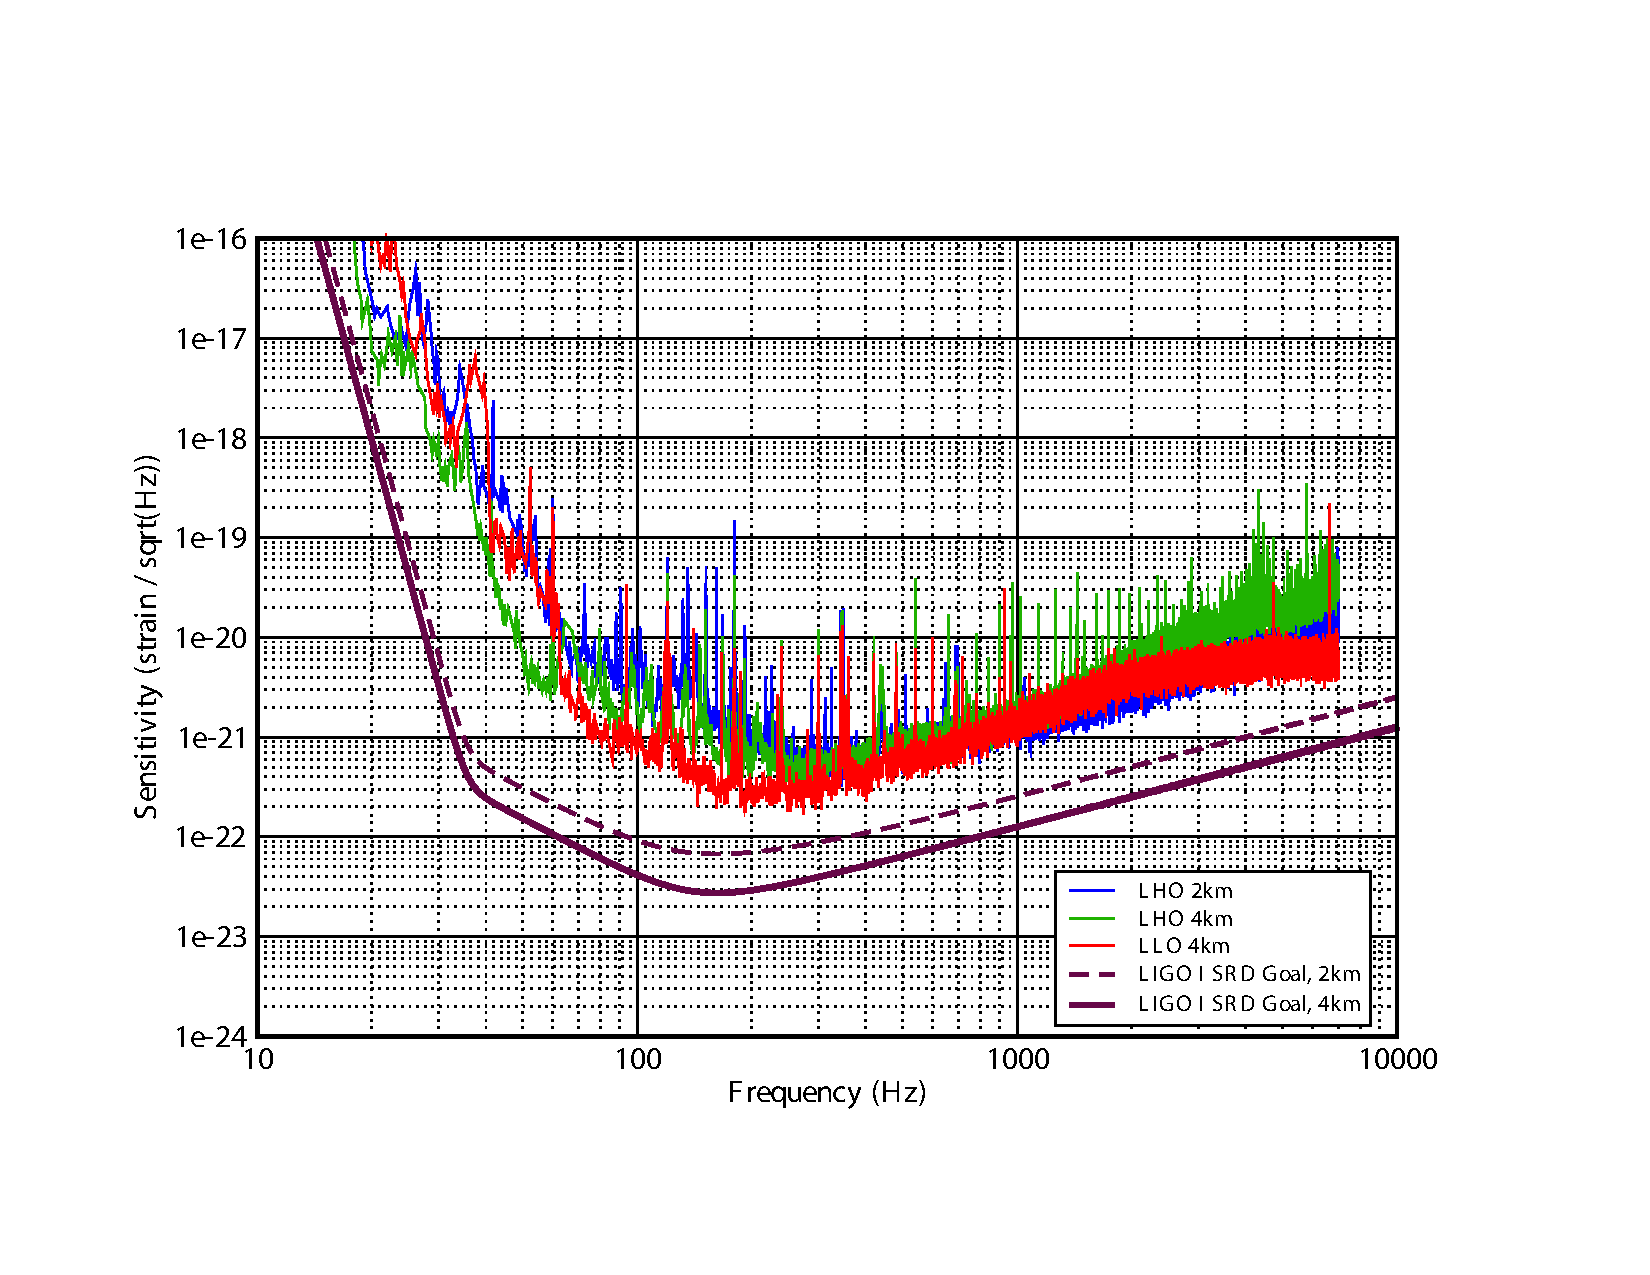
\includegraphics[width=\textwidth]{figures/pipeline/G030379-00}    
  \end{flushright}
  \caption{%
  Typical sensitivities of the three LIGO interferometers during the second
  LIGO science run\cite{s2noisecurve} shown as strain amplitude spectral
  density, $\tilde{h}/\sqrt{\mathrm{Hz}}$. The smooth solid curve shows the
  design sensitivity (SRD Goal) of the $4$~km interferometers and the smooth
  dashed curve shows the design sensitivity of the $2$~km interferometer.
  }
\label{f:s2noisecurve}
\end{figure}

\begin{figure}
\begin{center}
\hspace*{-0.2in}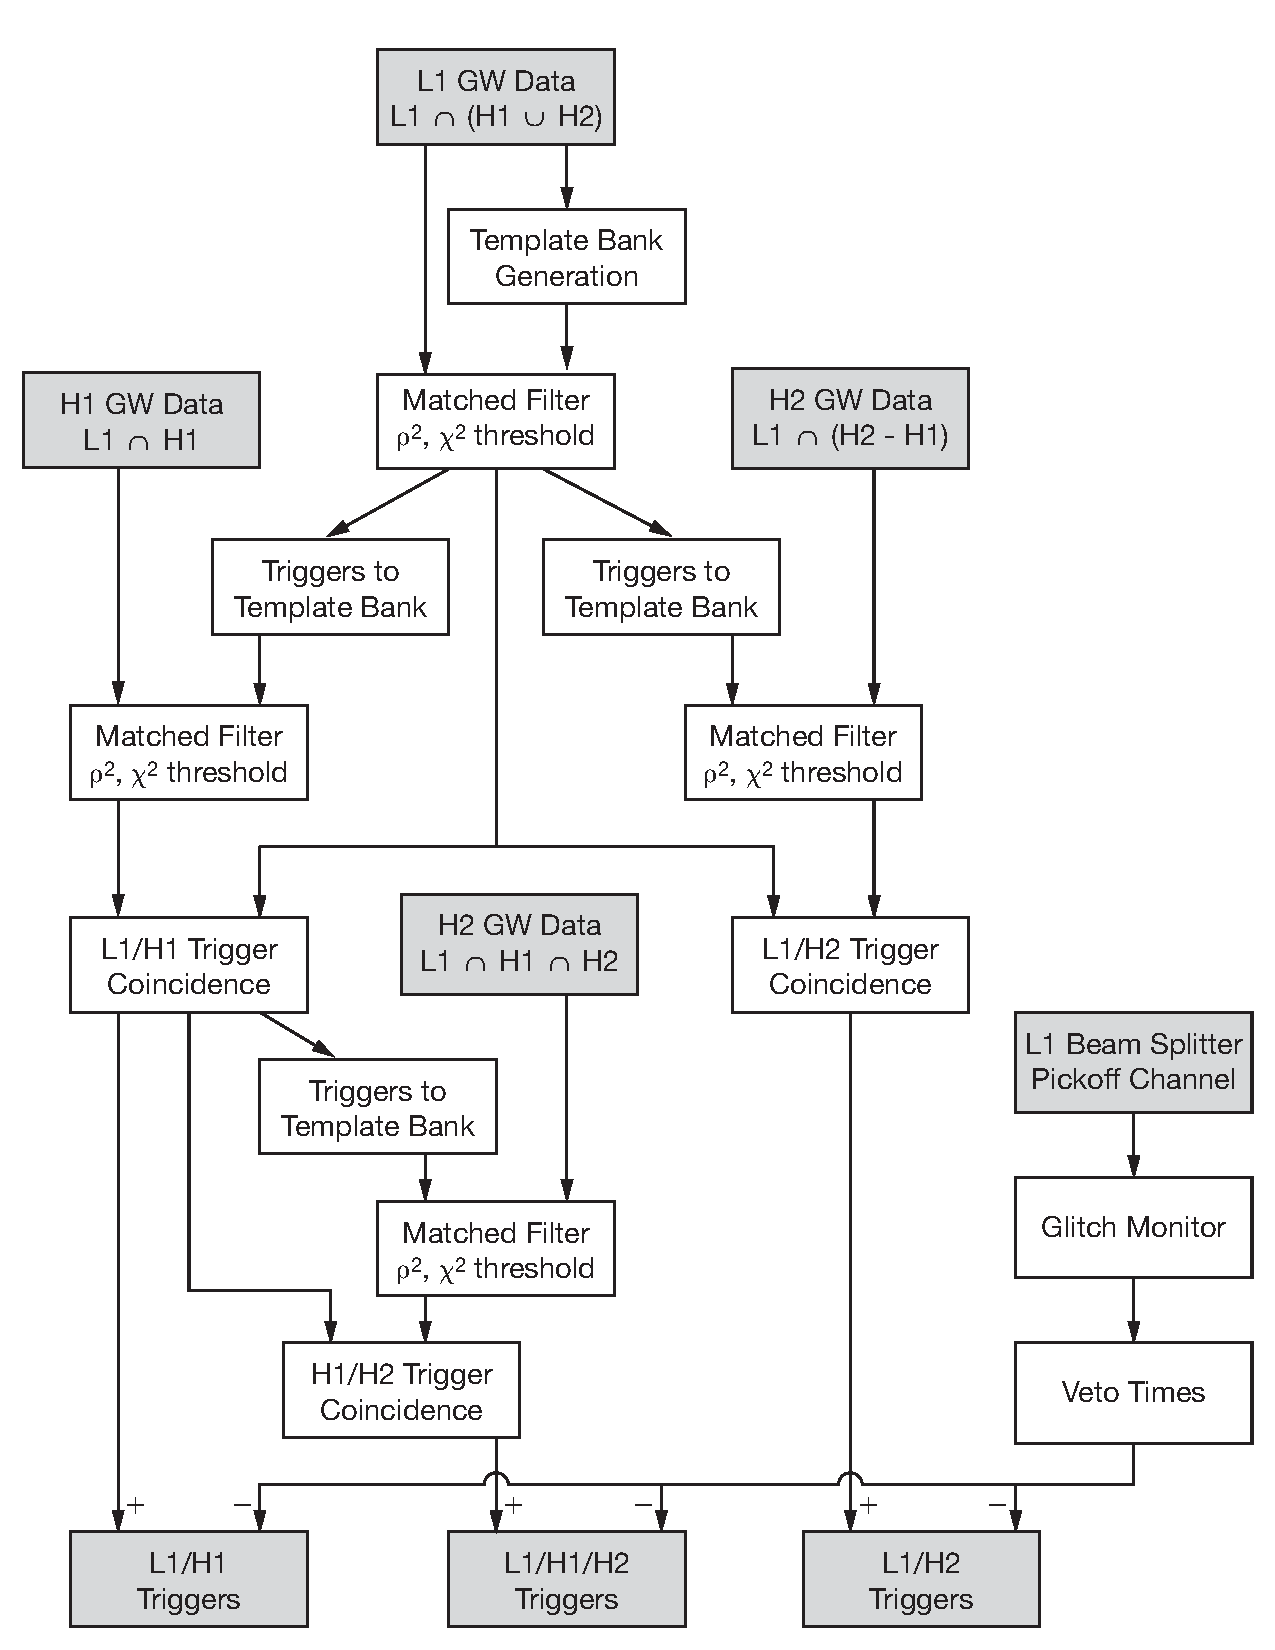
\includegraphics[width=\linewidth]{figures/pipeline/s2_pipeline}
\end{center}
\caption{\label{f:pipeline}%
The inspiral analysis pipeline used to determine the reported upper
limit. $\mathrm{L1} \cap (\mathrm{H1} \cup \mathrm{H2})$ indicates times when
the L1 interferometer was operating in coincidence with one or both of the
Hanford interferometers. $\mathrm{L1} \cap \mathrm{H1}$ indicates times when
the L1 interferometer was operating in coincidence with the H1 interferometer.
$\mathrm{L1} \cap (\mathrm{H2} - \mathrm{H1})$ indicates times when the L1
interferometer was operating in coincidence with only the H2 interferometer.
The outputs of the search pipeline are triggers that belong to one of the
two double coincident data sets or to the triple coincident data set.}
\end{figure}

The power spectral density (PSD) of the noise in the Livingston detector is
estimated independently for each L1 chunk that is coincident with operation of
a Hanford detector (denoted $\mathrm{L1} \cap (\mathrm{H1} \cup
\mathrm{H2}$)).  The PSD is used to lay out a template bank for filtering that
chunk, according to the parameters for mass ranges and minimal
match\cite{Owen:1998dk}. The data from the L1 interferometer for the chunk is
then filtered, using that bank, with a signal-to-noise threshold
$\rho_{\mathrm{L}}^\ast$ and $\chi^2$ veto threshold
$\chi^2_{\ast\mathrm{L}}$ to produce a list of triggers as described in
section~\ref{s:triggers}.  For each chunk in the Hanford interferometers, a
{triggered bank} is created by adding a template if it produced at least one
trigger in L1 during the time of the Hanford chunk.  This is used to filter
the data from the Hanford interferometers with signal-to-noise and $\chi^2$
thresholds specific to the interferometer, giving a total of six thresholds
that may be tuned.  For times when only the H2 interferometer is operating in
coincidence with L1 (denoted $\mathrm{L1} \cap (\mathrm{H2} - \mathrm{H1}$)
the triggered bank is used to filter the H2 chunks that overlap with L1 data;
these triggers are used to test for L1/H2 double coincidence.  All H1 data
that overlaps with L1 data (denoted $\mathrm{L1} \cap \mathrm{H1}$) is
filtered using the triggered bank for that chunk. For H1 triggers produced
during times when all three interferometers are operating, a second triggered
bank is produced for each H2 chunk by adding a template if it produced at
least one trigger found in coincidence in L1 and H1 during the time of the H2
chunk and the H2 chunk is filtered with this bank.  These triggers are used to
search for triple coincident triggers in H2.  The remaining triggers from H1
when H2 is not available are used to search for L1/H1 double coincident
triggers.


\section{Trigger Coincidence}
\label{s:coincidence}

For a trigger to be considered coincident in two interferometers, we demand
that it is observed in both interferometers within a temporal coincidence
window, $\delta t$, that allows for the error in measurement of the time of the trigger. Monte Carlo analysis with simulated signals suggests that we
cannot measure the time of the trigger to an accuracy of less than $1$~ms, so
we demand $\delta t = 1$~ms if the interferometers are located at the same
observatory. If the detectors are not co-located, we allow for the $10$~ms
light travel time between the LIGO observatories by demanding $\delta t =
11$~ms. We also demand that the waveform of the triggers are consistent by
requiring that the two mass parameters, $m_1$ and $m_2$, of the binary are
identical to within an error of $\delta m$.

\begin{figure}
  \vspace{5pt}
  \begin{flushright}
    \includegraphics[width=\textwidth]{figures/pipeline/gmst_dist_ratio}    
  \end{flushright}
  \caption{%
  The ratio of the known effective distance of an injected signal in the
  Hanford Observatory (LHO) to the known effective distance of an injected
  signal in the Livingston Observatory (LLO) as a function of Greenwich Mean
  Sidereal Time. The slight misalignment of the interferometers at the two
  different observatories due to the curvature of the earth causes the antenna
  pattern of the detectors to differ. As a result the distance at which a
  binary system appears is different in each detector, even in the absence of
  noise.  The ratio of effective distances can be significant, so this
  precludes the use of an amplitude cut when testing for inspiral trigger
  coincidence between different observatories.
  }
\label{f:gmst_dist_ratio}
\end{figure}
We now consider an amplitude cut on the signals. The Livingston and Hanford
detectors are not co-aligned. There is a slight misalignment of the detectors
due to the curvature of the earth and so the antenna patterns of the detectors
differ. This causes the measured amplitude of a gravitational wave to differ
between the sites. In the extreme case, it is possible for a binary to be
completely undetectable by the L1 detector, but still detectable by the H1 and
H2 detectors. For a given inspiral trigger, we measure the \emph{effective
distance} of the binary system. This is the distance at which an optimally
oriented binary would produce the observed signal-to-noise ratio.
Figure~\ref{f:gmst_dist_ratio} shows the ratio of effective distances between
the two LIGO observatories for the population of binary neutron stars
considered in the S2 analysis. The significant variation of the effective
distance precludes using a naive test for amplitude coincidence. It is
possible to obtain information about sky position from time delay between
sites to construct a more complicated amplitude cut, but this has not be used
in the S2 analysis.

In the case of triggers from the H1 and H2 interferometers that are coincident
in time and mass, we apply an amplitude cut that tests that the effective
distance of the triggers is coincident given the relative sensitivity of the
detectors, while allowing for error in this measurement which is determined by
Monte Carlo simulations.  When testing for triple coincident triggers we 
accept triggers that are coincident in the L1 and H1 detectors that are
\emph{not} present in the H2 detector \emph{if} the effective distance of the
trigger is further than the maximum distance of H2 at signal-to-noise ratio
$6$ at the time of the candidate trigger. Figure \ref{f:coinc_test} summarizes
the time, mass and distance coincidence test.  The final step of the pipeline
is to apply and auxiliary interferometer vetoes described in
section~\ref{s:vetoes}. 

The list of surviving candidate triggers is followed up by examining the raw
gravitational wave data, auxiliary interferometer channels and physical
environment monitoring channels to determine if the triggers are truly of
astrophysical origin.

\begin{figure}
\begin{center}
\hspace*{-0.2in}\includegraphics[width=\linewidth]{figures/pipeline/s2_coinc_test}
\end{center}
\caption{\label{f:coinc_test}%
The test to decide if a trigger in the first detector has a coincident 
trigger in the second detector. If detectors are at different sites, time and
mass coincidence are demanded. The effective distance cut is disabled by 
setting $\kappa = 1000$. If the detectors are at the same site, we ask if the
maximum distance to which H2 can see at the signal-to-noise threshold
$\rho_\mathrm{H2}^\ast$ is greater than the distance of the H1 trigger,
allowing for errors in the measurement of the trigger distance. If this is the
case, we demand time, mass and effective distance coincidence.  If distance to
which H2 can see overlaps the error in measured distance of the H1 trigger, we
search for a trigger in H2, but always keep the H1 trigger even if no
coincident trigger is found. If the minimum of the error in measured distance
of the H1 trigger is greater than the maximum distance to which H2 can detect
a trigger we keep the H1 trigger without searching for coincidence.}
\end{figure}

\section{Background Estimation}
\label{s:background}

Since we restrict the S2 analysis to coincident data and require that at least
two of the interferometers must be located at different observatories, we may
measure a background rate for our analysis. After generating triggers for each
interferometer, we slide the triggers from one observatory relative to the
other observatory and look for coincidences between the shifted and zero lag
triggers. The minimum slide length is chosen to be greater than the length of
the longest filter ($20$~seconds) so any coincident triggers detected must be due to background and
not astrophysical events. By examining the distribution of background events
in the $(\rho_\mathrm{H},\rho_\mathrm{L})$ plane we can attempt to determine
contours of constant false alarm rate in order to construct a combined
effective signal-to-noise ratio for a coincident trigger\cite{abbott2004a}.

\section{Detection Efficiency}
\label{s:eff}

In absence of detection, we will construct an upper limit on event rate.  To
do this, need to measure the detection efficiency of the analysis pipeline to
our population. A Monte Carlo method is used to measure this efficiency. We
simulate a population of binary neutron stars and \emph{inject} signals from
that population into the data from all three LIGO interferometers. The
injection is performed in software by generating an inspiral waveform and
adding it to interferometer data immediately after the raw data is read from
disk. We inject the actual waveform that would be detected in a given
interferometer accounting for both the masses, orientation, polarization, sky
position and distance of the binary, the antenna pattern and calibration of
the interferometer into which this signal is injected.  The effectiveness of
software injections for measuring the response of the instrument to an
inspiral signal is validated against \emph{hardware injections}\cite{hw} where
an inspiral signal is added to the interferometer control servo during
operation to produce the same output signal as a real gravitational wave.  The
data with injections is run through the full analysis pipeline to produce a
list of inspiral triggers. The detection efficiency of the pipeline,
$\epsilon$, is the ratio of the number of detected signals to the number of
injected signals.

\Chapter{Hardware Signal Injections}
\label{ch:hardware}
% $Id$

%\section{Motivation for Hardware Injections}
%\label{s:motivation}
Gravitational radiation incident on the LIGO interferometers from an
inspiralling binary will cause the test masses to move relative to each other.
This produces a differential change in length of the arms as described in
section \ref{s:effect}.  \emph{Injection} is the process of adding a waveform to
interferometer data to simulate the presence of a signal in the noise. We use
injections to measure the performance of the binary inspiral analysis
pipeline as described in section \ref{s:eff}.  \emph{Software injections},
which add a simulated signal to the data after it has been recorded, are used
for efficiency measurements. Since they performed \emph{a posteriori} the
interferometer is not affected while it is recording data.  Alternatively, a
simulated signal can be added to the interferometer control system to make the
instrument behave as if an inspiral signal is present.  The interferometer
Length Sensing and Control system has excitation points which allow arbitrary
signals to be added into the servo control loops or to the drives that control
the motion of the mirrors\cite{LIGOS1instpaper}.  We call this \emph{hardware
injection}; the data recorded from the instrument contains the simulated
signal. Figure \ref{f:ifo_inj} shows the hardware injection points on a
schematic diagram of the interferometer and length sensing and control loop.

Analysis of hardware injections allows us to ensure that the analysis pipeline
is sensitive to real inspiral signals and validates the software injections
used to test the pipeline efficiency.  In order to perform an accurate upper
limit analysis for binary inspirals, we must measure the efficiency of our
pipeline. That is, we inject a known number of signals into the pipeline and
determine the fraction of these detected.  Injecting signals into the
interferometer for the duration of a run is not practical and would
contaminate the data, so we use the analysis software to inject inspiral
signals into the data.  By comparing software and hardware injections we
confirm that software injections are adequate to measure the efficiency of the
upper limit pipeline.

Hardware injections provide a very complete method of testing the inspiral
detection pipeline. By recovering the physical parameters of an injected
signal, we test our understanding of all aspects of the pipeline, including
the instrumental calibration, the filtering algorithm and veto safety. We
injected inspiral signals immediately after the first LIGO science run (S1) in
September 2002. The resulting data was analyzed using the
software tools used to search for real signals.  In this chapter, we describe
the results of analysis of the S1 hardware injections. The analysis pipeline
used in S1 differs from that used in S2\cite{LIGOS1iul}. Here we are examining
the response of the filtering code to the hardware injections, however, and so
the differences between the S1 and S2 pipelines are unimportant.

\section{Injection of the Inspiral Signals}
\label{s:injecting}

To inject the signals, we generate the interferometer strain $h(t)$ produced
by an inspiralling binary using the restricted second order post-Newtonian
approximation in the time domain\cite{Blanchet:1996pi}.  The LSC calibration group
supplies a transfer function $T(f)$ which allows us to construct a signal
$g(t)$ that produces the desired strain when it is injected into the
interferometer.  The transfer function $T(f)$ should be identical to the
actuation function $A(f)$ described in section \ref{ss:calibration}, however
in S1 this was simplified to contain only the pendulum response of the mirrors,
given by 
\begin{equation}
T(f) = \frac{L}{C}\frac{f^2}{f_0^2}
\end{equation}
where $L$ is the length of the interferometer, $C$ is the calibration of the
excitation point in nm/count and $f_0$ is the pendulum frequency of the test
mass. Damping is neglected as it is unimportant in the LIGO frequency band.
The code used to generate the hardware injections is the same as that used
for software injections; only the transfer function used to generate the
injected signal differs since we are injecting into the control signal $g$
rather then the error signal $v$.

During S1, we injected signals corresponding to an optimally oriented binary.
Injections of two $1.4\,M_\odot$ neutron stars at distances from $10$ kpc to
$80$ kpc were used to test the neutron star analysis. 
We also injected signals from a $1.4,\,4.0\,M_\odot$ binary and several
$1.4,1.4\,M_\odot$ binaries at closer distances.  These signals were injected
into the differential mode servo and directly into an end test mass drive.

\section{Detection of the Injected Signals}
\label{s:detection}

Figure \ref{f:inj_snr} shows the events generated by processing 4000 seconds
of data from the Livingston 4 km interferometer (L1) on 10 September 2002
during the post-run hardware injections.

The first set of injections were large amplitude signals used to verify the
inspirals were being correctly injected. We ignore these and concentrate on
the second set, which were at more appropriate distances.  We only consider
the 1.4 solar mass inspiral injections, as the 1.4,4.0 injection lies
outside the template bank space used in the S1 binary neutron star analysis.

It can be seen that all of the hardware injections are identified as candidate
events since they have high signal-to-noise ratios and values of the $\chi^2$
test lower than $5$, which was the threshold used in the S1 analysis
pipeline\cite{LIGOS1iul}. Some of the 1.4,4.0 injections are also flagged
for further investigation as they cause templates inside the bank to ring, but
have high $\chi^2$ values as they are not exactly matched.

Since we know the exact coalescence time of the injected waveform, we can
compare this with the value reported by the search code and ensure that the
search code is reporting the correct time.  The known and measured parameters
for the second set of $1.4,1.4\ M_\odot$ injections are shown in table
\ref{t:triggers}. The raw data is resampled to $4096$ Hz before being
filtered. For each of the signals injected, we were able to detect the
coalescence time of the injection to within one sample point of the correct
value at $4096$ Hz, which is consistent with the expected statistical error
and confirms that the pipeline has not introduced any distortion of the
signals.


\section{Checking the Instrumental Calibration}
\label{s:calibration}

Calibration measurements of the interferometers were performed before and
after the run; these are the reference calibrations. In general, the
calibration changes due to changes in the alignment on time scales of minutes.
This variation is encoded in the parameter $\alpha$ which is
monitored using a sinusoidal signal injected into the
detector (see section \ref{ss:calibration}). $\alpha$ is used as input
to the data analysis pipeline and varied between $0.4$ and $1.4$ during S1.
Data in S1 was analyzed in 256 second segments.  For each 256 seconds of data
starting at time $t_0$, we construct the calibration, $R(f;t_0)$ by using
$\alpha(t_0)$ and a reference calibration.  $R(f;t_0)$ is then used to
calibrate the 256 seconds of data.

Figure \ref{f:calibration} shows a set of injections into the Livingston
interferometer analyzed with different calibrations generated by varying the
value of $\alpha$. We expect that the signal-to-noise varies quadratically and
the effective distance varies linearly with changes in $\alpha$\cite{Allen:1996}.
This is confirmed by the injections.  There is no single value of $\alpha$
that gives the correct effective distance for all the injections; this is
consistent with the estimated systematic errors in the calibration.
Unfortunately the calibration line was not present during the time the
hardware injections were performed, so we cannot directly compare a measured
calibration with the result of the injections.

\section{Safety of Vetoes}
\label{s:safety}

During construction of the the inspiral pipeline we considered using inspiral
triggers found in auxiliary interferometer channels as vetoes on triggers in
the gravitational wave channel. Concern was raised that a real inspiral signal
may couple between these channels and a real signal may be inadvertently
vetoed.  To check this, we examined coupling between the channels at the time
of an injection.  Figure \ref{f:veto_safe} shows the power spectra of the
gravitational wave channel, LSC-AS\_Q, and the auxiliary channels that we
considered using as vetoes during S1: LSC-AS\_I, LSC-REFL\_I and
LSC-REFL\_Q.  The injected inspiral signal can clearly be seen coupling
to the auxiliary channel LSC-AS\_I, but there is no obvious coupling
between the injected signal and LSC-REFL\_I or LSC-REFL\_Q. This
led us to discard LSC-AS\_I as a possible veto channel in the S1
analysis. Similar studies have been performed for the S2 data when auxiliary
channels are proposed as veto channels.

\newpage

\begin{figure}[p]
  \vspace{5pt}
  \begin{flushright}
    \includegraphics[width=\textwidth]{figures/hardware/ifo_inj}    
  \end{flushright}
  \caption[Schematic of LIGO Interferometer Showing Injection Points]{%
  A schematic diagram of the LIGO interferometer showing the injection points
  used in S1 hardware injections. Inspiral signals were injected either
  directly into the end test mass drive of one arm or into the differential
  mode servo, and this into both arms. Care was taken to ensure that the
  correct transfer function, $T(f)$, was used in each case.
  }
\label{f:ifo_inj}
\end{figure}

\begin{figure}[p]
  \vspace{5pt}
  \begin{flushright}
    \includegraphics[width=\textwidth]{figures/hardware/inj_snr}    
  \end{flushright}
  \caption[Candidate Events from Hardware Injections]{%
The candidate events generated by processing 4000 seconds of data from the
Livingston 4 km interferometer through the S1 analysis pipeline.  This data
included two sets of injections; the known coalescence times are indicated by
the dashed vertical lines. The signal-to-noise ratio is plotted and the value
of the $\chi^2$ veto is shown next to the candidate event.
  }
\label{f:inj_snr}
\end{figure}

\begin{table}[p]
  \begin{flushright}
  \begin{tabular}{l|l|c|c}
  End time of Injection&End Time of Detection&$\rho$&$\chi^2$\\
  \hline
  $04:35:12.424928$ & $04:35:12.424927$ & $11.623546$ & $1.653222$ \\
  $04:36:42.424928$ & $04:36:42.425171$ & $20.230101$ & $1.671016$ \\
  $04:38:12.424928$ & $04:38:12.424927$ & $37.488770$ & $0.443966$ \\
  $04:39:42.424928$ & $04:39:42.424927$ & $69.815262$ & $1.375486$ \\
  \end{tabular}
  \end{flushright}
  \caption[Hardware Injections Found by the Analysis Pipeline]{%
  Hardware injection events found by the inspiral analysis pipeline. End time
  of injection is the known end time of the injected signal and end time of
  detection is the end time of the signal as reported by the analysis
  pipeline. Times are Universal Time (UTC) on 10 September 2002. The values of
  signal-to-noise ratio $\rho$ and $\chi^2$ veto are given for each event.
  }
\label{t:triggers}
\end{table}

\begin{figure}[p]
  \vspace{5pt}
  \begin{flushright}
    \includegraphics[width=\textwidth]{figures/hardware/calibration}    
  \end{flushright}
  \caption[Study of Calibration Using Hardware Injections]{%
  Each curve corresponds to a hardware injection at the given GPS time. We
  re-analyze each injection with different calibrations to show how the
  detected quantities vary with $\alpha$. The upper plot shows the ratio of
  signal-to-noise ratio, $\rho$, to its maximum value, $\rho_{\mathrm{max}}$.
  The lower plot shows ratio of the detected distance to the known distance of
  the hardware injection.
  }
\label{f:calibration}
\end{figure}

\begin{figure}[p]
  \vspace{5pt}
  \begin{flushright}
    \includegraphics[width=\textwidth]{figures/hardware/veto_safe}    
  \end{flushright}
  \caption[Study of Veto Safety Using Hardware Injections]{%
  Power spectra of the gravitational wave channel LSC-AS\_Q and the auxiliary
  channels LSC-AS\_I, LSC-REFL\_I and LSC-REFL\_Q during a 
  hardware injection. The broad peak in the spectrum is the inspiral signal
  and the two power spectra taken at subsequent times show it sweeping across
  the band as the frequency of the inspiral signal increases with time.
  }
\label{f:veto_safe}
\end{figure}





%\chapter{Searches for Binary Neutron Star Coalescence}
%\label{ch:bns}
%% $Id$

\section{Target Sources}

\section{Data Quality Checks and Vetoes}

\section{Parameter Tuning}

\section{S1 Search Results}

\subsection{Triggers and Event Candidates}

\subsection{Error Analysis}

\section{S2 Search Results}

\subsection{Background Estimation}

\subsection{Triggers and Event Candidates}

\subsection{Error Analysis}


\Chapter{The Rate of Binary Black Hole MACHO Inspirals in the Halo}
\label{ch:result}
% $Id$

\section{Introduction}

Motivation for search: dark matter problem in the galaxy, microlensing
results, Nakamura proposal that MACHOs may be (B)BHs. Predicted rate is
$5\times10^{-2}\times2^{\pm 1}$ events/yr/galaxy is higher than BNS rate.
Waveforms well modelled, same pipeline as S2 BNS. Brief description of sciruns
with reference to instument paper and S2 BNS paper.

\section{Population}

Review Ioka et al paper on BBH formation in the early universe. Density of
local dark matter. Review population models used and make some plots of MACHO
distribution.

\section{Analysis Pipeline and Tuning}

Refer to findchirp paper for trigger generation, gwdaw proceedings and S2
paper for description of pipeline. Give brief description of triggered search
pipeline. Coincidence criteria. Details of tuning MACHO pipeline.

\section{Search Results}

Background, triggers, upper limit. Error analysis for MACHOs.

\section{Conclusions}

Detection? Rate? How close to predicted rate? How long until astrophysically
interresting result?


\Chapter{Conclusion}
\label{ch:conclusion}
In the current era of gravitational-wave astrophysics we are moving beyond first direct detections and first multimessenger observations, to now making routine discoveries that deepen our understanding of the compact objects in our cosmic neighborhood. The LIGO-Virgo gravitational-wave detector network has detected 52 confirmed binary merger observations so far, and the detection rate has only accelerated as improved detector sensitivity extends our reach deeper into the universe. From the two observed binary neutron star mergers, our knowledge of the dynamics of these events and of neutron star physics has grown dramatically. They have provided confirmation of binary neutron star mergers as a source of short gamma-ray bursts, and also as important sites of heavy element production through $r$-process nucleosynthesis that can help explain observed chemical abundances. They have also shown that it is possible to measure the tidal information in a gravitational-wave signal to meaningfully update our constraints on the nuclear equation of state. As the LIGO-Virgo detectors approach their design sensitivity, and as third-generation detectors begin to come online, we expect to see many more binary neutron star mergers in the coming years. We anticipate that these new detections will provide even further insights into the physics of neutron stars.

In this thesis we have studied binary neutron star mergers, through a combination of observations and computational modeling. Specifically we explore the ability of a gravitational-wave analysis to extract physical parameters of the binary system, and of the neutron stars involved in the merger. We investigate the impact of multimessenger information on a gravitational-wave analysis, and we study the measurability of the nuclear equation of state, both now and in the future.

We have presented an analysis of the binary neutron star merger GW170817 informed by electromagnetic distance measurements of its identified host galaxy, and we demonstrated that using an independent distance measurement in a gravitational-wave analysis can break the distance-inclination degeneracy to allow for much tighter constraints on the inclination angle of the binary. We find our improved measurement of the inclination supports models for a structured relativistic jet and its afterglow emission being viewed off-axis.

We have presented measurements of the tidal deformabilities and radii of the neutron stars in GW170817. Our analysis imposed a physical constraint to require that both neutron stars obey the same equation of state, and we used a prior on the leading order tidal parameter constructed to contain all physical models of the equation of state without biasing the measurement toward any particular model. We note that the methodology we employed could be adapted for the analysis of future binary neutron star merger events with similar masses. We find our results are broadly consistent with several other studies~\cite{Abbott:2018exr,Radice:2018ozg,Coughlin:2018fis,Capano:2019eae} which employed various methods to measure the tidal deformabilities and radii in their own analyses of GW170817.

We have presented a likelihood model developed for \textit{PyCBC Inference} that uses the relative binning parameter estimation technique to reduce computational cost for potential multimessenger gravitational-wave sources. We extended the work of previous implementations to make our relative likelihood model a coherent network statistic so that it can additionally measure sky locations. We validated the relative model on populations of simulated binary neutron star and simulated neutron star--black hole merger signals, and we showed that it is possible to seed the relative analysis with the best-fit template parameters from a low-latency search pipeline. We found that the parameter estimation for all signals in our simulated populations completed in less than 20 minutes, with sky localization and intrinsic parameter estimates that are comparable to analyses done with a standard non-relative likelihood.

We have presented a comprehensive study of the future prospects for a precise equation of state measurement from Advanced LIGO and Cosmic Explorer. We explored the measurability of the equation of state across the full parameter space allowed by combined constraints from astrophysical observations and nuclear experiments. We showed that a precision threshold for measurements to distinguish between substantially similar theoretical models for the equation of state is equivalent to measuring the radius of a 1.4\msun\ neutron star to better than $2\%$, and we presented a framework for combining individual equation of state measurements across entire populations to produce a combined, high-precision measurement. We found it is unlikely that Advanced LIGO will achieve $2\%$ precision in the next observing runs given current estimates of the merger rate for binary neutron stars, however Cosmic Explorer will measure the equation of state to better than $1\%$ within one year of operation. Our framework can be directly applied to any future signals from binary neutron star mergers, and we anticipate that the resulting precise knowledge of the true equation of state will be invaluable for efforts to model these merger events and their associated kilonovae.

\clearpage
\bibliographystyle{unsrt}
\bibliography{references}
\addcontentsline{toc}{chapter}{\numberline {Bibliography}}

\clearpage
\birthplacedate{Lucknow, India \>\>September 2, 1987}
\collegewherewhen{%
\>Birla Institute of Technology \& Science, Pilani, India \>\>2005--2009, \>B.E.~(Hons)\\
\>\syr	\>\>2009--2014, \>Ph.D.}

\newpage
\null\vskip1in%
\begin{center}
{\Large\bf Curriculum Vitae}
\end{center}
\vskip 2em
\begin{tabbing}
\tabset
Title of Dissertation\\
\>Topics in Gravitational-Wave Astronomy \\
\end{tabbing}
\vskip 1em

\begin{startvita}
\end{startvita}

\renewenvironment{thebibliography}[1]%
  {\begin{list}{\labelenumi\hss}%
     {\usecounter{enumi}\setlength{\labelwidth}{3em}%
      \setlength{\leftmargin}{5em}}}%
  {\end{list}}
\renewcommand{\bibitem}[1]{\item\label{#1}\relax}%
\renewcommand{\theenumi}{\arabic{enumi}}%
\begin{publications}
\putbib[papers]
\end{publications}

\begin{honorarysocieties}
2003 \> UWM Chancellor's Graduate Student Fellowship\\
2003 \> UWM Dissertator Fellowship\\
2002 \> Physics Graduate Student Trust Fund Award\\
2002 \> UWM Chancellor's Graduate Student Fellowship\\
2002 \> UWM Graduate School Fellowship\\
2001 \> Papastamatiou Scholarship\\
1999 \> Institute of Mathematics and Its Applications Prize\\
1997 \> Stroud Book Prize for Theoretical Physics
\end{honorarysocieties}

\finishvita
\end{document}
